% !TEX program = arara
% arara: pdflatex
% arara: biber
% arara: pdflatex
% arara: pdflatex
% arara: clean: { files: [ Paper.out ] }
% arara: clean: { files: [ Paper.aux, Paper.bbl ] }
% arara: clean: { files: [ Paper.bcf, Paper.blg ] }
% arara: clean: { files: [ Paper.log, Paper.run.xml ] }
% arara: clean: { files: [ Paper.toc, Paper-blx.bib ] }
% 

\documentclass{Paper}
\usepackage{todonotes}
\usepackage{xcolor}
\usepackage{pgf-pie}
\usepackage{pgfplots}
\usepackage{float}
\usepackage{textcomp}
\usepackage{subfigure}
\usepackage{filecontents}
\usepackage{pgfplots, pgfplotstable}
\usepgfplotslibrary{statistics}
% define custom colours
\definecolor{greenOfApproval}{HTML}{009933}
\definecolor{redOfDisapproval}{HTML}{cc0000}
\definecolor{yellowOfBrevity}{HTML}{000000}
\definecolor{purpleOfLengthiness}{HTML}{6600cc}

\begin{document}

\maketitle

% % % % %

\tableofcontents
\clearpage
	
\section{Abstract}
	\todo{Autor: Berna, überarbeitet: Jana}

Das Ziel dieses Projekts ist festzustellen, wie sich menschliche Zeitwahrnehmung in der Virtual Reality durch visuelle und akustische Zeitgeber manipulieren lässt.  Dazu wurden 48 Versuchspersonen in einer virtuellen Umgebung sowohl schnellen als auch langsamen Zeitgebern ausgesetzt, um danach Wahrnehmungen, Einschätzungen und generelle Eindrücke in Fragebögen und Zeiteinschätzungstest abfragen zu können. Die meisten Ergebnisse sind nicht aussagekräftig. Auffälligkeiten sind \textbf{hier Ergebnisse einfügen, sofern welche vorhanden}

\section{Einleitung}
\todo{Autor: Kim}
\subsection{Einstieg}

In den letzten Jahrhunderten unverkennbar zu beobachten ist ein enormer Wandel unserer Gesellschaft auf technischer sowie sozialer Ebene.
Eine Zunahme der Relevanz des Begriffes „Zeit“ ist durch die öffentlichen Diskussionen über Stress, Burn-Out oder dergleichen zu beobachten.
Immer mehr Menschen der arbeitenden Gesellschaft leiden unter diesen Krankheiten, die auf „zu wenig Zeit“ zurückzuführen sind. Das zunehmende Interesse der Themen Effizienz, Schnelligkeit und Leistung ist außerdem unübersehbar. Die Gesellschaft versucht immer schneller und immer mehr Arbeiten in einer kürzeren Zeit zu erledigen. Dies ist ganz offensichtlich auch auf die Industrialisierung und auf das zunehmende Tempo der Gesellschaft zurückzuführen. \cite{Wallish2003} Wo früher noch Tage auf die Antwort eines Briefes gewartet wurde, ist es heute möglich innerhalb weniger Minuten ganze Arbeitsschritte oder Anweisungen via Email zu kommunizieren und anschließend die erwarteten Leistungen zu erbringen.
Des Weiteren lässt sich beobachten, dass die Arbeits-und Schlafzeiten der arbeitenden Bevölkerung massiv gesenkt wurden. \cite{DeutscheSozialgeschichte}
\\
Aufgrund von weniger Schlafzeiten ergibt sich nun die Bildung der Freizeit und somit die Notwendigkeit des Zeitmanagements. Jeder versucht seine Tage optimal zu nutzen und einzuteilen, um noch genug Zeit für die Freizeit und Familie zu haben. Des Weiteren schaffen auch die neuen Entwicklungen der Industrialisierung wie Handy, Mikrowelle, Computer und weitere technische Erfindungen mehr Zeit für jeden Einzelnen. Dennoch sind Versuche, die Zeit durch immer effizientere und „zeitsparendere“ Abläufe zu bändigen nur Scheinerfolge: Die Zeit vergeht trotzdem gleichförmig und schleichend unaufhaltsam und unwiderruflich weiter. \cite{Wallish2003} Es besteht also ein hohes Interesse in der Erforschung dieses Gebietes, um die Zeit, die jedem Einzelnen zur Verfügung steht, optimal zu nutzen.

Dennoch steht uns immer noch derselbe biologische Apparat zur Verfügung. Zeit vergeht also trotzdem gleichförmig und einheitlich. Doch die Frage ist: Ist das wirklich so? Vergeht die Zeit immer gleich schnell oder gibt es bestimmte Indikatoren, die uns die Zeit als schneller oder langsamer vergehend vorkommen lassen? Kann man das Zeitempfinden also beeinflussen?

\subsection{Fragestellung}
Dies führt zu der Forschungsfrage: \textbf{Kann man das Zeitempfinden in der Virtuellen Welt durch bestimmte Zeitgeber manipulieren?}\\
Zeitgeber sind Phänomene der allgemeinen Lebenswelt und physische Kräfte, die uns unter Ausschluss der Uhrzeit die Zeit vorgeben.
In diesem Projekt wurde eine beschleunigte und verlangsamte Gravitation als visueller und das Ticken einer Ampel als auditiver Zeitgeber verwendet. Die verwendete virtuelle Welt ist an Alltagssituationen angelehnt.
%Nach Ablauf der unsere Versuchsstrecke wurde die Versuchsperson mithilfe eines Fragebogens zu seinen Eindrücken in der virtuellen Welt befragt und durch die „Four Alternative Forced Choice“ - Methode „gezwungen“, die einzelnen erlebten Szenarien nach ihrer Dauer zu sortieren. So erhofften wir uns herauszufinden, ob eine der erlebten Manipulationen die Zeitwahrnehmung der Versuchsperson rafft oder streckt. Mithilfe von Statistik (siehe \ref{Methodik}) ließ sich nun herausfinden, ob eines der Manipulations-Szenarien überproportional auffällig von allen Versuchspersonen als kürzer bzw. länger eingestuft wurde als andere Szenarien und wir somit eine Manipulation der Zeit erzeugen konnten. 


Ein weiterer Fokus dieser Arbeit liegt auf dem Einfluss der VR auf das menschliche Zeitempfinden und der Frage, ob sich menschliche Zeiteinschätzung nach dem Aufenthalt in der VR verändert.  
%\textbf{Unterscheidet sich die Zeiteinschätzung der einzelnen Versuchspersonen vor und nach dem Aufenthalt in der Virtuellen Welt?} Verändert also das Erlebnis, sich in einer nicht reellen Welt zu befinden das Zeitempfinden?


%Unter Betrachtung des Spaßfaktors, der auch einen erheblichen Einfluss auf die Zeitwahrnehmung nimmt, wurden alle Versuchspersonen zusätzlich gebeten, die Dauer bestimmter Zeitintervalle jeweils vor und nach dem Befinden in der virtuellen Welt einzuschätzen.


 %Wenn die Versuchspersonen der Meinung waren, dass die Zeitintervalle vorbei waren (40 Sekunden, 40 Sekunden mit Unterhaltung, 30 Sekunden ) sollten sie es durch ein Zeichen kenntlich machen. Zusätzlich wurde sich bei einem der Einschätzungsintervalle mit den Versuchspersonen unterhalten, um ebenfalls herauszufinden, ob Ablenkung einen Einfluss auf die Zeitwahrnehmung nehmen konnte.


\subsection{Hypothesen}

Bezüglich unserer zwei Forschungsschwerpunkte haben wir folgende Hypothesen erstellt:
\begin{enumerate}
\item ,,Visuelle und auditive Zeitgeber verändern das Zeitempfinden der Versuchsperson in der virtuellen Welt''
%Wir vermuten, dass die Manipulation der Zeitgeber in einer virtuellen Welt die Zeitwahrnehmung verändert und die Zeit somit schneller oder langsamer vergeht.

\item ,,Der Spaßfaktor in der virtuellen Welt hat einen Einfluss auf die Zeitwahrnehmung der Versuchsperson.''

%Der Spaßanteil, den jeder während einer Aktion erlebt, hat großen Einfluss auf die Zeitwahrnehmung und kann die vergangene Zeit raffen oder im Falle von geringem Spaßfaktor strecken.


\item ,,Das Befinden in der virtuellen Welt verändert das Zeitempfinden nach Rückkehr in die reale Welt''

%Wir vermuten, dass das Befinden in der virtuellen Welt das Zeitempfinden kurzzeitig beeinflussen und verändern kann.
\end{enumerate}


%Das Ziel der Arbeit ist es, die Hypothesen zu be- oder widerlegen. 
%Das Belegen der Hypothesen wäre ein wichtiger Wegweiser für weitere Forschungen in diese Richtung.\\
%Das Ziel dieser Arbeit ist es dieses Forschungsfeld anzustoßen und Freiraum für weitere Experimente zu schaffen.

\subsection{Forschungsstand}
Diese Arbeit bezieht sich auf und orientiert sich an verschiedenen Studien zur Zeitwahrnehmung und Zeitmanipulation in der virtuellen Welt. \\
Die Studie ,,Could Virtual Reality Help Manipulate Time Perception?'' untersucht, ob die Veränderung der Sonnenzirkulation in der VR einen Einfluss auf die Zeitwahrnehmung nehmen kann. Auch diese Forschungsgruppe benutzte verschiedene Zeitgeber, um eine Manipulation des Zeitempfindens hervorzurufen: die Sonne ohne Bewegung, die Sonne im normalen 24-Stunden-Zyklus und 
ein Tages- bzw. Sonnenzyklus doppelter Geschwindigkeit (gemessen an der Realität).
 Die Versuchspersonen wurden in drei Gruppen aufgeteilt. Die erste Gruppe sollte passiv auf einem Stuhl sitzen, die zweite sollte eine sprachliche, kognitive Aufgabe lösen und die dritte eine ,,räumliche''.\\
Diese Forschungsgruppe kam zu folgendem Ergebnis: Wenn die Versuchspersonen passiv blieben, überschätzten sie die Zeit und die Sonnenbewegungen hatten einen großen Einfluss auf ihre Zeitwahrnehmung. Wenn sie aber währenddessen mit einer Aufgabe beschäftigt waren, unterschätzten sie die Zeit, die in der VR vergangen war und die Sonnenzyklen hatten keinen Einfluss. \cite{Device&Systems} Daraus wird deutlich, dass kognitive und räumliche Aufgaben die Versuchspersonen zu sehr ablenken. Daher sind in diesem Projekt keine kognitiven oder räumlichen Aufgaben integriert und verwendete Zeitgeber können ihre Wirkung entfalten.\\
Pascal Wallisch' wissenschaftlicher Bericht ,,Zeiterleben in der Tempogesellschaft'' enthält weitere Einflussfaktoren, welche zu beachten sind.  \\
Wallisch beschreibt, \glqq dass das menschliche Zeitempfinden, insbesondere die Empfindung von Dauer von allen möglichen Faktoren abhängig ist\grqq . \cite{Wallish2003} S. 27 \\
Für unser Experiment ist es von bedeutender Wichtigkeit, dass keiner der Versuchspersonen in seiner Zeitempfindung durch Faktoren beeinflusst wird, um sicherzustellen, dass korrekte Ergebnisse resultieren.
Mithilfe eines Fragebogens werden Faktoren und Einflüsse ausgeschlossen bzw. in die Auswertungsergebnisse miteinbezogen und gesondert betrachtet, die von Wallisch’s beschrieben wurden. 
So können abweichende Ergebnisse begründet und auf veränderte Einflussfaktoren Rücksicht genommen werden.\\
Zu diesen Einflüssen gehören unter anderem Intelligenz, Alter, Geschlecht, Drogen-und Medikamenteneinflüsse, Müdigkeit (bedingt, da Müdigkeit nur die Ereignis-Fusions Schwelle senkt und nicht direkt die Zeitwahrnehmung verändert ( \ref {Kapitel 3.3})), Körpertemperatur, Gehirnschäden und psychische Erkrankungen.\\
Weiterhin wurden die Ergebnisse des Artikels ,,Warum Jahre rasen und Sekunden schleichen'' berücksichtigt. Dieser veranschaulicht, dass auch das Spaßempfinden einen Einfluss auf die Zeitwahrnehmung nimmt.\cite{Welt24}


\subsection{Aufbau der Arbeit}
Dieses Paper stellt einen Versuch dar, sich der Möglichkeit der Zeitmanipulation zu nähern, indem zunächst - nach einem kleinen historischen Überblick über die Entwicklung von Zeit - das Ziel der Arbeit, sowie die Vorgehensweise des Experiments erläutert wird. Des Weiteren wird auf den Forschungsstand in diesem Gebiet der Zeitforschung eingegangen und Foschungshypothesen werden aufgeführt. Aus diesen wird eine sinnvolle Methodik abgeleitet, vorgeschlagen und durchgeführt, insofern dies mit den gegebenen Mitteln machbar erschien. Deren Resultate werden in einem abschließenden Teil im Sinne der Fragestellung und der Hypothesen aufgeführt, interpretiert, diskutiert und zukunftsorientiert betrachtet.


\section{Methode}
        \todo{Autor: Nizan \& Alina}
        \subsection{Methodik}
Die wissenschaftliche Methode des Experiments war die Grundlage unseres Projekts, anhand der wir unsere Leitfrage und Hypothesen auf ihren Wahrheitsgehalt untersuchten um Zusammenhänge darzustellen.
Es galt bestimmte Untersuchungs-Anordnungen zu berücksichtigen, um so die Erhebung von Daten zur Zeitwahrnehmung zu sichern, aufbauend auf bereits bekannten Erfahrungswerten. \textbf{Von welche Methode wird hier geredet?}
               
Die Forschung über menschliches Verhalten birgt ethische Schwierigkeiten. Besonders wenn die Manipulationen die Persönlichkeit eines Menschen langfristig prägen oder beeinflussen. Deshalb wurde sich bei der Themenwahl strickt an die ethischen Richtlinien gehalten, um die Sicherheit der Versuchspersonen zu gewährleisten. 
Die Versuchspersonen wurden im Vorfeld weitestgehend über den Ablauf des Verfahrens, die vorhersehbaren Unannehmlichkeiten und die Risiken aufgeklärt. Es bestand jederzeit die Möglichkeit das Experiment abzubrechen.

%Beim wissenschaftlichen Arbeiten gilt es einige grundsätzlichen Kriterien zur Sicherung der Qualität einzuhalten. Diese sind Ehrlichkeit, Objektivität, Überprüfbarkeit, Logik, Originalität, Validität und Verantwortung auf deren Einhaltung wir großen Wert gelegt haben.\\
%\textbf{Welcher Bezug haben Ehrlichkeit, Objektivität, Überprüfbarkeit, Logik, Originalität, Validität und Verantwortung mit dem Experiment?}


        \subsection{Versuchspersonen}

Das Projekt wird mit insgesamt 48 Versuchspersonen unterschiedlicher akademischer Grade und Berufe  durchgeführt, wobei 35 männlich und 13 weiblich sind und sich im Alter zwischen 17 und 80 Jahren befinden. Von diesen wurden fünf Versuchspersonen aufgrund von unvollständigen Angaben von der Auswertung ausgeschlossen. \\
Die insgesamt 24 verschiedenen Reihenfolgen der Szenarien konnten mit dieser Anzahl an Versuchspersonen realisiert werden, sodass jeweils zwei Versuchspersonen eine konkrete Reihenfolge erlebten.\\
Alle Versuchspersonen haben nach eigenen Angaben normale oder mit Brille bzw. Kontaktlinsen korrigierte Sehkraft und normales Farbsehen. Personen mit psychischen Erkrankungen, Gehirnschäden oder schlechten Deutschkenntnissen wurden nicht für das Experiment aufgenommen. Die Versuchspersonen waren bezüglich der experimentellen Hypothesen unwissend und unterschrieben vor der Teilnahme eine schriftliche Einverständniserklärung. %über alle Risiken und datenschutzrechtlichen Informationen.
Es wurde keine Entschädigung angeboten. 
                %\footnote{$()$}
               
        \subsection{Apparaturen}
Zwei Räume wurden für die Durchführungen des Experiments genutzt. Im ersten Raum, in dem der erste und letzte Teil des Experiments stattfand, wurden die Befragungen und Zeiteinschätzungs-Tests gemacht.
Zu der dort vorliegenden Probandenmappe gehören folgende Dokumente:\\               
         	(1) Einverständniserklärung, (2) \glqq Fragebogen B\grqq, (3) \glqq Fragebogen A\grqq, (4)
                Mehrfach-Wortschatz-Intelligenztest und (5) \glqq Fragebogen C\grqq.
% Diese wurden, in Klemmbrettern geordnet, für die Durchläufe mit den Versuchspersonen vorbereitet. \\
Im zweiten Raum wurden die VR-Experimente durchgeführt, in dem die Versuchsperson auf einem Drehstuhl saß.\textbf{Zusatz: Conrtoller, PC (Specs?), Monitor etc.}

        \subsection{Prozedur}
%Das Experiment fand in einer Laborsituation unter kontrollierten Bedingungen statt. Die
%Ergebnisse des Experiments sind unabhängig vom Versuchsleiter zustande gekommen.//
Der Ablauf des Experiments bestand aus den drei Phasen. Phase 1: Intelligenztest und erste Zeiteinschätzung, Phase 2: Navigation durch die virtuelle Testumgebung, Phase 3: Zweite Einschätzung.


\subsubsection{Intelligenztest und erste Zeiteinschätzung}
Jeder Durchlauf begann mit einer Einweisung durch die Räumlichkeiten. Der erste Teil des
Experiments fand in ''Raum 1'' statt. Der Versuchsleiter und
die Versuchsperson saßen sich gegenüber an einem Tisch. Der Versuchsperson unterschrieb eine
Einverständniserklärung. \textbf{nötig?}
Ein Zeiteinschätzungs-Test wurde durchgeführt, in dem die
Versuchsperson 40 Sekunden ohne Hilfsmittel und ohne sich zu unterhalten einschätzen sollte.
Das Ergebnis wurde von einem der anwesenden Versuchsleiter anhand einer Stoppuhr
gemessen und auf dem ''Fragebogen B'' erfasst. \\
Der Versuchsperson wurde ''Fragebogen A'' ausgehändigt. Es sollte angegeben werden (1) ob die zu testende Person unter Drogeneinflüssen steht, (2) wie der aktuelle Müdigkeitswert ist, (3) ob und an welchen Gehirnschäden oder psychischen Erkrankungen die Person leidet und (4) welche die
Muttersprache der Versuchsperson ist.

Ein Intelligenztest (MWT-B) wurde durchgeführt. Bei dem angewandten Intelligenztest handelte es sich um den psychologisch anerkannten ''Mehrfach-Wortschatz-Test (MWT-B)'', entwickelt von Siegfried Lehrl \cite{MWT-B}, den wir nach Empfehlungen des Psychologie Studenten Till Rachwitz, der sich auf die Durchführung von Intelligenztests spezialisiert hat, gewählt haben. Dieser begründete die Wahl dieses Tests damit, dass er simpel und kurz durchzuführen ist. Er bietet einen groben Überblick über die allgemeine Intelligenz einzelner Personen. Im MWT-B gilt es aus 37 Wortreihen, bestehend aus jeweils vier fiktiven und einem existierendem deutschen Wort, das korrekte Wort zu finden und durchzustreichen. Es gab keine zeitliche Begrenzung und keine Hilfestellung.

Ein erneuter Zeiteinschätzungs-Test wurde durchgeführt, in dem die Versuchsperson 40 Sekunden abschätzen und sich gleichzeitig mit den Versuchsleiter unterhalten sollte. \\
Anschließend wurde die Körpertemperatur der Versuchsperson mit Hilfe des Infrarot-Thermometers am Ohr gemessen und anschließend ein 30 Sekunden
Zeiteinschätzungs-Test ohne Gespräch durchgeführt. Alle Ergebnisse der Zeiteinschätzungen und die
Körpertemperatur wurden von dem Versuchsleiter auf dem vorgedruckten ''Fragebogen B''
notiert. Die Versuchsperson hatte keine Einsicht in die Ergebnisse.

\subsubsection{Navigation durch die virtuelle Testumgebung}
Der zweite Teil findet in ''Raum 2'' statt. Die Versuchsperson bekam die Anweisung, sich auf einen Drehstuhl zu setzen. Weitere Anweisungen für die Durchführung vom Experiment waren: (1) Die Fortbewegung findet mittels eines Xbox-Controllers statt, (2) Man kann sich frei durch die Welt bewegen, (3) Anhand der VR-Brille kann man sich umsehen, (4) Man sollte sich an die allgemeinen Verkehrsregeln halten, (5) Die Umgebung sollte für spätere Befragungen einprägt werden.

Zu Beginn des Experiments wurde die Zeit von dem Moment des Loslaufens bis zu dem End-Schild gestoppt. %, um zu wissen wie lange die Versuchsperson für die gesamte Strecke der vier Szenarien benötigt. 
Die insgesamt vier Szenarien bildeten die virtuelle Welt und bestanden aus vier Ampelkreuzungen, die der realen Welt durch visuelle und auditive Aspekte nachgebaut wurden.

\begin{figure}[H]
	\centering
	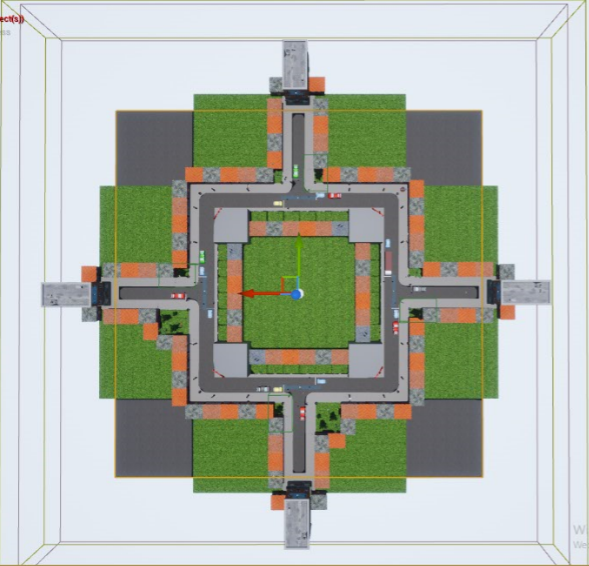
\includegraphics[scale=0.7]{../Bilder/map.png}
	\caption{Ansicht der virtuellen Welt von oben, in der an jeder Ampel eines der Szenarien stattfindet.}
	\label{img:map}
\end{figure}

An jeder Ampelkreuzung gab es einen manipulierten Zeitgeber, der die
Zeitwahrnehmung beeinflussen soll. Alle vier Szenarien gleichen sich optisch, haben aber unterschiedliche Zeitgeber. 
\begin{itemize}
\item{(a) Ampelphase an einem LKW - schnelles Ticken} 
\item{(b) Ampel mit Vogel und Menschen - langsames Ticken}
\item{Ampel neben einem schaukelndem Kind mit rosa Shirt - schnelles Schaukeln} 
\item{Ampel mit Heißluftballon-Plakat bei einem schaukelndem Kind mit grünem Shirt - langsames Schaukeln.}
\end{itemize}


\begin{figure}[H]
	\subfigure[Ampelphase an einem LKW]{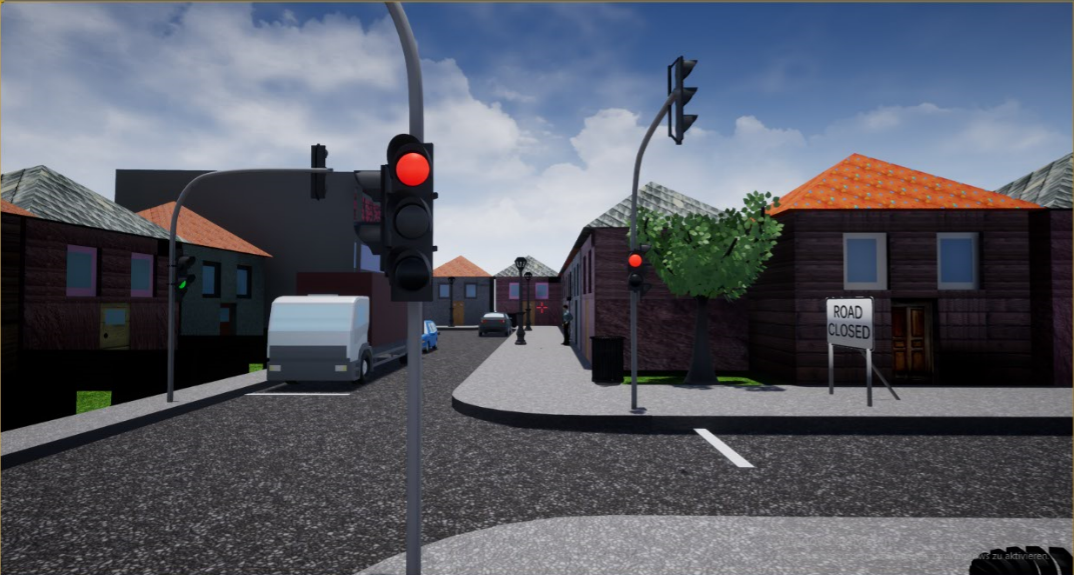
\includegraphics[width=0.5\textwidth]{../Bilder/a.png}}
	\subfigure[Ampelphase mit Vogel und Menschen]{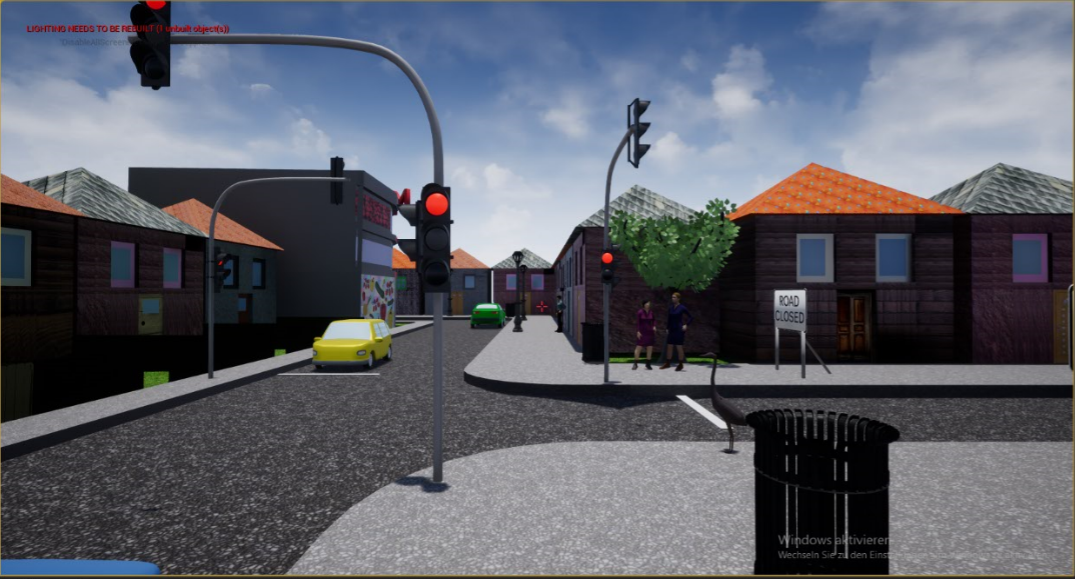
\includegraphics[width=0.5\textwidth]{../Bilder/b.png}}
	\caption{Ampelphasen an zwei Kreuzungen}
	\label{img:ampelphasen-1}
\end{figure}

\begin{figure}[H]
	\subfigure[Ampel neben einem schaukelndem Kind mit rosa Shirt]{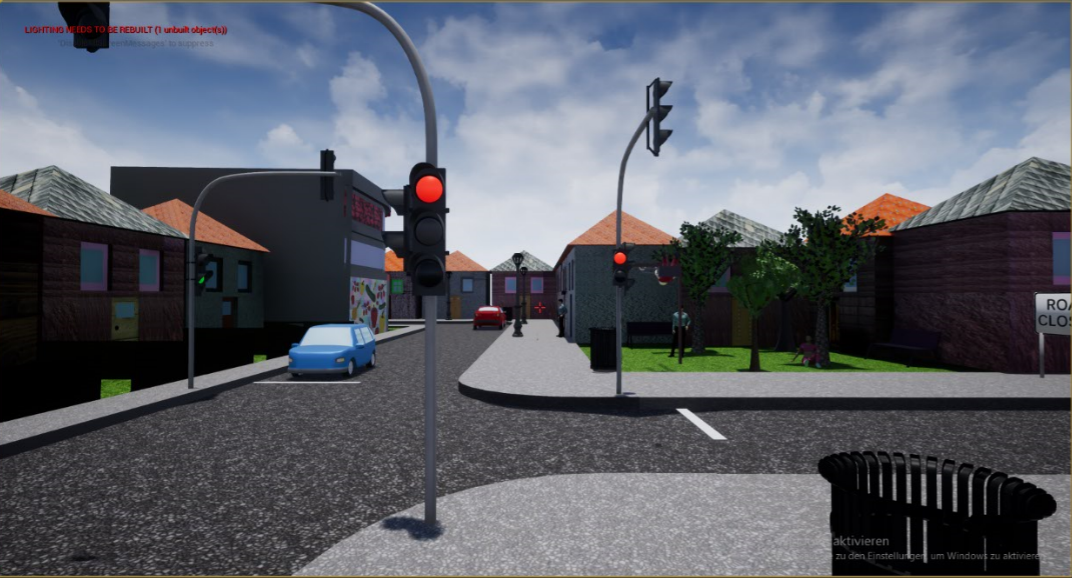
\includegraphics[width=0.5\textwidth]{../Bilder/c.png}}
	\subfigure[Ampel neben einem schaukelndem Kind mit grünem Shirt]{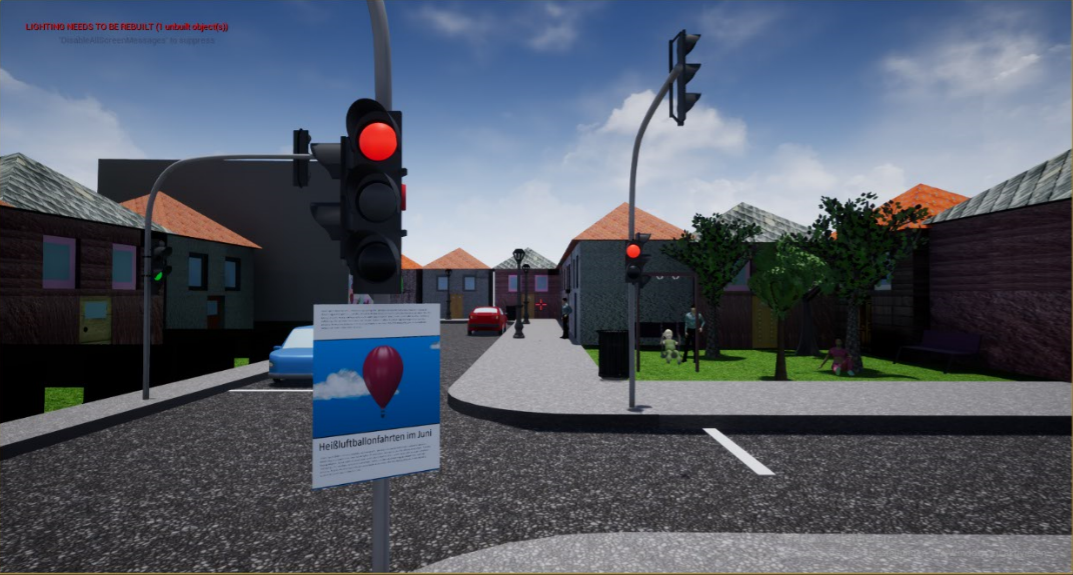
\includegraphics[width=0.5\textwidth]{../Bilder/d.png}}
	\caption{Ampelphasen an den anderen Kreuzungen}
	\label{img:ampelphasen-2}
\end{figure}

Die Wartezeit an den Ampelkreuzungen war vorgegeben und konnte nicht frühzeitig beendet werden. Die Versuchsperson durchlief die virtuelle Welt einmal und ohne zeitliche Begrenzung oder Unterbrechungen. Die Geschwindigkeit in der die Welt durchlaufen wurde, konnte die
Versuchsperson selbst anhand des Controllers regulieren. Die Versuchsleiter konnten das
Geschehen in der VR über die Bildschirme beobachten.

\subsubsection{Zweite Einschätzung}
Nach der VR wird die Versuchsperson wieder im ersten Raum auf verschiedene Dinge getestet.
40 Sekunden ohne
Unterhaltung wurden abgeschätzt und vom Versuchsleiter erfasst. Die Versuchsperson erhielt
'Fragebogen C' und sollte angeben: (1) die geschätzte Dauer von den einzelnen Szenarien
(2), die besten und schlechtesten empfundenen Szenarien, (3) die empfundene Dauer in
der virtuellen Welt, (4) den eigens empfundenen Spaßfaktor, (5) auffallende
Besonderheiten in der virtuellen Welt und (6) eine Einschätzung, worum es in dem
Experiment ging.//

Es wurde ein Zeiteinschätzungstest von 40 Sekunden mit Gespräch durchgeführt und vom
Versuchsleiter notiert. Darauf folgte ein weiterer Zeiteinschätzungstest von 30 Sekunden und
ohne Gespräch.//
Die Versuchsperson durfte ihre Zeiteinschätzungs-Ergebnisse auf Wunsch erfahren, sowie das Ergebnis vom
Intelligenztest. Räume und Klemmbretter für die nächste Versuchsperson wurden vorbereitet.

        \subsection{Begründung des Aufbaus und Wartezeiten}



Der Aufbau der Welt ist statisch, sodass die verschiedenen Reihenfolgen der Szenarien durch Teleports realisiert werden. Um die Erfahrung und Beeinflussung der virtuellen Testumgebung auf die Versuchspersonen nicht zu stören, sehen alle Ecken der Karte/Teleportpunkte gleich aus. Die Versuchsperson läuft über eine entsprechend positionierte Triggerbox und merkt auf diese Weise nicht, dass sie an eine andere Stelle der Karte teleportiert wird.\\
Die visuelle Zeitmanipulation wird durch ein schaukelndes Kind realisiert, das durch ensprechende Animationen den Eindruck macht, schneller (Szenario \textbf{c}) oder langsamer (Szenario \textbf{d}) zu schaukeln als es in der Realität möglich ist. Diese Szenarien sind von an der Ampel stehende Versuchspersonen gut zu beobachten und können so auf Versuchspersonen wirken.\\
Das gleichmäßige schnelle (Szenario \textbf{a}) oder langsame (Szenario \textbf{b}) Ticken der Fußgängerampel stellt die auditive Manipulation dar. Um die Erinnerung an die Szenarien zu erleichtern werden verschiedenen auffällige Objekte in den jeweiligen Szenarien verwendet: ein LKW (Szenario \textbf{a}) und ein Fischreiher auf dem Fußgängerweg (Szenario \textbf{b}).
Die Wartezeit jedes Szenarios beträgt 18 Sekunden und basiert auf zuvor gemessenen realen Ampelzeiten. Über eine Triggerbox wird die Ampelschaltung aktiviert, sobald sich die Versuchsperson entsprechend genähert hat. Die Wartezeit ist einerseits kurz genug, sodass bei den Versuchspersonen keine Ungeduld hervorgerufen wird und andererseits lang genug, dass die Versuchspersonen die Möglichkeit haben sich von ihrer Umgebung beeinflussen zu lassen. 


 \section{Ergebnisse}
\subsection{Streudiagramme}
Zu Beginn der Auswertung wurde versucht, Variablenpaare unserer gesammelten Werte in Beziehung zueinander zu setzen und dafür Streudiagramme zu erstellen. Zuvor erfolgte bereits eine Auseinandersetzung damit, welche Faktoren die Zeitwahrnehmung beeinflussen können: so kann sie z.B. mit jungem/höherem Alter, mit einer tiefen/hohen Körpertemperatur, einer niedrigen/ hohen Intelligenz, bei Müdigkeit sowie unter Männern und Frauen variieren. Herausgestellt wurden diese Beeinflusser von Pascal Wallisch in seinem Paper "`Zeiterleben in der Tempogesellschaft'' \cite{Wallisch2003}: "`Ein wesentlicher Punkt ist, dass das menschliche Zeitempfinden, insbesondere die
Empfindung von Dauer von allen möglichen Faktoren abhängig ist.''.\\
Erste Zeiteinschätzungen werden in Relation zu Alter, Intelligenz, Körpertemperatur und Müdigkeit der Versuchspersonen gestellt.
Die Streudiagramme sind gruppiert nach den Einschätzungen, die Versuchspersonen entweder \textit{ohne Gespräch} (Diagramme \textbf{X} bis \textbf{X}) oder \textit{mit Gespräch} (Diagramme \textbf{X} bis \textbf{X}) absolviert haben.
Rote Kreise stellen die weiblichen Versuchspersonen dar, blaue Kreise die männlichen.
%%%%%%%%%%%%%%%%%%%%%%%%% SCATTERPLOT ALTER
\begin{figure}[H]
\begin{minipage}[t]{0.49\linewidth}
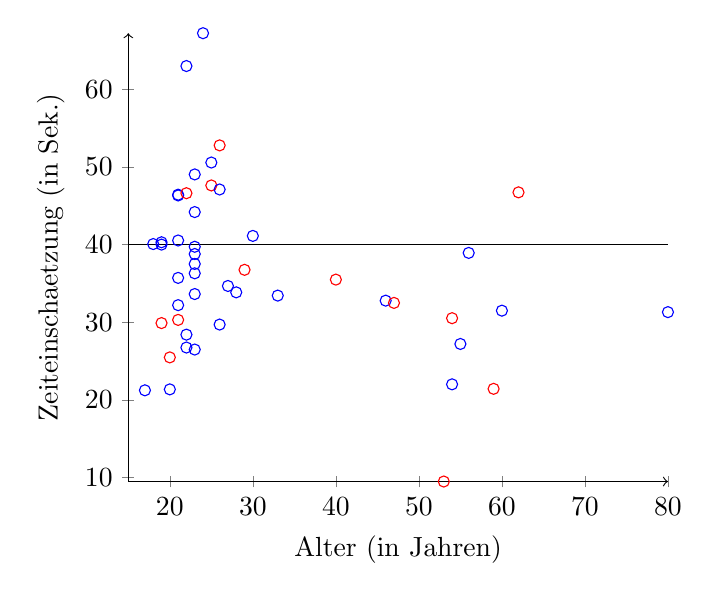
\begin{tikzpicture}
\begin{axis}[%
scatter/classes={%
    a={mark=o,draw=blue},
    b={mark=o,draw=red}},
    axis lines=middle,
    axis line style={->},
    x label style={at={(axis description cs:0.5,-0.1)},anchor=north},
    y label style={at={(axis description cs:-0.1,.5)},rotate=90,anchor=south},
    xlabel={Alter (in Jahren)},
    ylabel={Zeiteinschaetzung (in Sek.)}]
    % Orientierungslinie
        \addplot[domain=15:80]{40};
        % Scatter
    \addplot[scatter,only marks,%
    scatter src=explicit symbolic]%
table[meta=label] {
x y label
17 21.23 a
18 40.07 a
19 40.00 a
19 40.3 a
19 29.89 b
20 21.35 a
20 25.47 b
21 46.33 a
21 40.53 a
21 35.71 a
21 46.43 a
21 32.20 a
21 30.3 b
22 46.62 b
22 63.00 a
22 26.74 a
22 28.4 a
23 36.30 a
23 33.63 a
23 26.48 a
23 39.72 a
23 37.51 a
23 44.19 a
23 49.04 a
23 38.79 a
24 67.23 a
25 50.57 a
25 47.62 b
26 52.78 b
26 29.70 a
26 47.10 a
27 34.67 a
28 33.85 a
29 36.75 b
30 41.12 a
33 33.43 a
40 35.49 b
46 32.78 a
47 32.49 b
53 9.48 b
54 30.52 b
54 22 a
55 27.2 a
56 38.93 a
59 21.42 b
60 31.49 a
62 46.73 b       
80 31.3 a
        };
\end{axis}
\end{tikzpicture}
\caption{Zeiteinschätzung von 40 Sekunden ohne Gespräch nach Alter}
\label{Zeit40sek}
\end{minipage}
\hfill
\begin{minipage}[t]{0.49\linewidth}
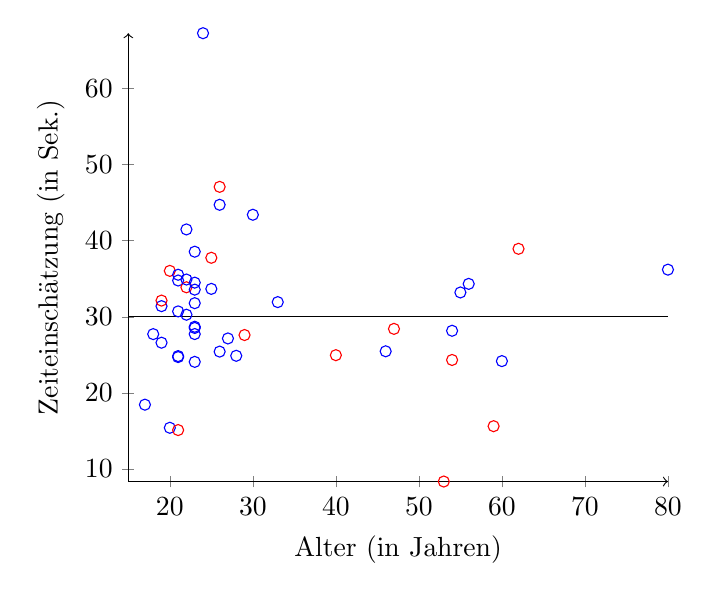
\begin{tikzpicture}
\begin{axis}[%
scatter/classes={%
    a={mark=o,draw=blue},
    b={mark=o,draw=red}},
    axis lines=middle,
    axis line style={->},
    x label style={at={(axis description cs:0.5,-0.1)},anchor=north},
    y label style={at={(axis description cs:-0.1,.5)},rotate=90,anchor=south},
    xlabel={Alter (in Jahren)},
    ylabel={Zeiteinschätzung (in Sek.)}]
   
    % Orientierungslinie
        \addplot[domain=15:80]{30};
        % Scatter
    \addplot[scatter,only marks,%
    scatter src=explicit symbolic]%
table[meta=label] {
x y label
17 18.44 a
18 27.72 a
19 26.59 a
19 31.4 a
19 32.13 b
20 15.40 a
20 36.04 b
21 34.77 a
21 35.53 a
21 24.83 a
21 30.71 a
21 24.70 a
21 15.1 b
22 33.88 b
22 41.49 a
22 30.27 a
22 34.9 a
23 28.69 a
23 34.49 a
23 24.07 a
23 31.79 a
23 27.73 a
23 28.53 a
23 33.57 a
23 38.56 a
24 67.30 a
25 33.67 a
25 37.76 b
26 47.09 b
26 25.42 a
26 44.73 a
27 27.15 a
28 24.87 a
29 27.60 b
30 43.42 a
33 31.93 a
40 24.95 b
46 25.46 a
47 28.41 b
53 8.33 b
54 24.32 b
54 28.16 a
55 33.2 a
56 34.33 a
59 15.61 b
60 24.17 a
62 38.94 b       
80 36.2 a
        };
\end{axis}
\end{tikzpicture}
\caption{Zeiteinschätzung von 30 Sekunden ohne Gespräch nach Alter}
\label{Zeit30sek}
\end{minipage}
\end{figure}

%%%%%%%%%%%%%%%%%%%%%%%%%%%%%%%%% HISTO ALTER %%%%%%%%%%%%%%%%%%%%%
\begin{figure}[H]
\begin{filecontents}{data.csv}
dist

21.23
40.07
40.00
40.3
29.89
21.35
25.47
 46.33
  40.53
 35.71
 46.43
32.20
 30.3
 46.62
 63.00
 26.74
 28.4
 36.30
 33.63
 26.48
 39.72
37.51
 44.19
 49.04
38.79
 67.23
 50.57
47.62
52.78
 29.70
 47.10
 34.67
33.85
36.75
 41.12
 33.43
 35.49
 32.78
 32.49
 9.48
 30.52
 22
  27.2
 38.93
 21.42
 31.49
46.73
 31.3
\end{filecontents}
\begin{minipage}[t]{0.49\linewidth}
\begin{tikzpicture}
\begin{axis}[
    ybar,
    ymin=0
]
\addplot +[
    hist={
        bins=10,
        data min=0.5,
        data max=50
    }   
] table [y index=0] {data.csv};
\end{axis}
\end{tikzpicture}
\caption{Anzahl der Personen(y), welche die jeweilige Zeiteinschätzung(x) angaben - 40 Sekunden ohne Gespräch nach Alter.}
\label{HistZeit40sek}
\end{minipage}
\hfill
\begin{filecontents}{data.csv}
dist
 18.44
 27.72
 26.59
 31.4
 32.13
 15.40
 36.04
 34.77
 35.53
 24.83
 30.71
 24.70
 15.1
 33.88
 41.49
 30.27
 34.9
 28.69
 34.49
 24.07
 31.79
 27.73
 28.53
 33.57
 38.56
 67.30
 33.67
 37.76
 47.09
25.42
44.73
 27.15
 24.87
 27.60
 43.42
 31.93
 24.95
 25.46
 28.41
 8.33
 24.32
 28.16
 33.2
 34.33
 15.61
 24.17
38.94
 36.2
\end{filecontents}
\begin{minipage}[t]{0.49\linewidth}
\begin{tikzpicture}
\begin{axis}[
    ybar,
    ymin=0
]
\addplot +[
    hist={
        bins=10,
        data min=0.5,
        data max=50
    }   
] table [y index=0] {data.csv};
\end{axis}
\end{tikzpicture}
\caption{Anzahl der Personen(y), welche die jeweilige Zeiteinschätzung(x) angaben - 30 Sekunden ohne Gespräch nach Alter.}
\label{HistZeit30sek}
\end{minipage}
\end{figure}

%%%%%%%%%%%%%%%%%%%%%%%%%%%%%%%%%%%%%%%%%%%%%%%%%%%%%%%% HISTO ALTER%%%%%%

Zunächst wird überprüft, ob das Alter auch in unserem Experiment Einfluss auf die Fähigkeit, Zeiten richtig einzuschätzen, hatte, jedoch ergeben die Werte der geschätzten Zeiten von 40 und 30 Sekunden (jeweils ohne Ablenkung) kein eindeutiges Bild. Auch wenn die Ausreißer im Diagramm unbeachtet bleiben, ist keine Abhängigkeit zwischen den Variablen "`Zeiteinschätzung'' und "`Alter'' zu erkennen. Zusätzlich in keine Auffälligkeit zwischen den Schätzungen männlicher und weibliche Versuchsperson zu sehen.

\todo{prozentsatz}



%%%%%%%%%%%%%% SCATTERPLOT INTELLIGENZ
\begin{figure}[H]
\begin{minipage}[t]{0.49\linewidth}
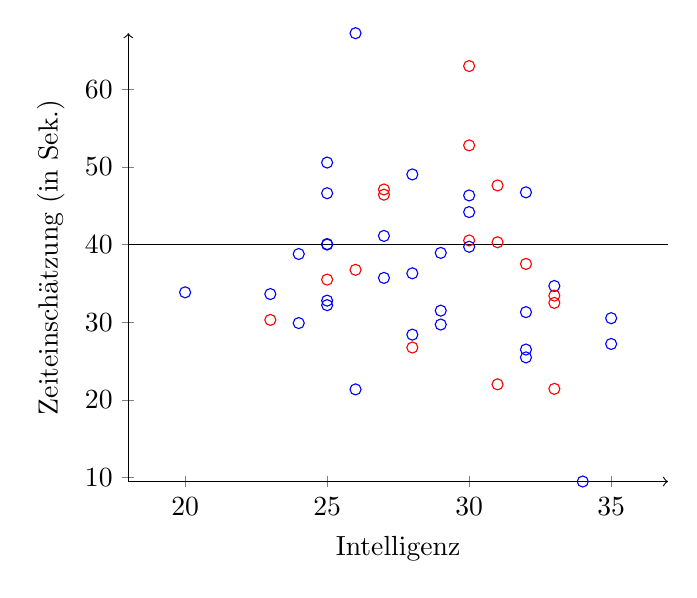
\begin{tikzpicture}
\begin{axis}[%
scatter/classes={%
    a={mark=o,draw=blue},
    b={mark=o,draw=red}},
    axis lines=middle,
    axis line style={->},
    x label style={at={(axis description cs:0.5,-0.1)},anchor=north},
    y label style={at={(axis description cs:-0.1,.5)},rotate=90,anchor=south},
    xlabel={Intelligenz},
    ylabel={Zeiteinschätzung (in Sek.)}]
  \addplot[domain=18:37]{40};
    \addplot[scatter,only marks,%
    scatter src=explicit symbolic]%
table[meta=label] {
x y label
20 33.85 a
23 30.3 b
23 33.63 a
24 29.89 a
24 38.79 a
25 40.07 a
25 40.00 a
25 32.20 a
25 46.62 a
25 50.57 a
25 35.49 b
25 32.78 a
26 21.35 a
26 67.23 a
26 36.75 b
27 35.71 a
27 46.43 b
27 47.10 b
27 41.12 a
28 26.74 b
28 28.4 a
28 36.30 a
28 49.04 a
29 29.70 a
29 38.93 a
29 31.49 a
30 46.33 a
30 40.53 b
30 63.00 b
30 39.72 a
30 44.19 a
30 52.78 b
31 22 b
31 40.3 b
31 47.62 b
32 25.47 a
32 26.48 a
32 37.51 b
32 46.73 a
32 31.3 a
33 34.67 a
33 33.43 b
33 32.49 b
33 21.42 b
34 9.48 a
35 30.52 a
35 27.2 a
    };
\end{axis}
\end{tikzpicture}
\caption{Zeiteinschätzung von 40 Sekunden ohne Gespräch nach Intelligenz}
\label{Zeit40sekInt}
\end{minipage}
\hfill
\begin{minipage}[t]{0.49\linewidth}
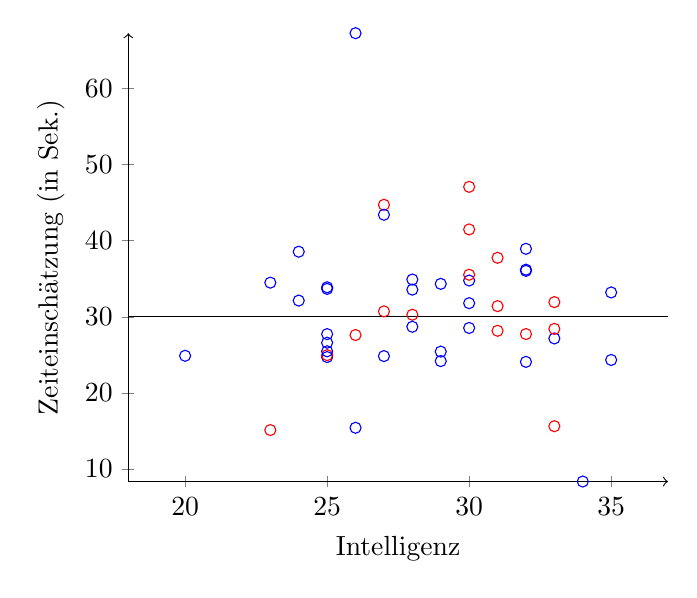
\begin{tikzpicture}
\begin{axis}[%
scatter/classes={%
    a={mark=o,draw=blue},
    b={mark=o,draw=red}},
    axis lines=middle,
    axis line style={->},
    x label style={at={(axis description cs:0.5,-0.1)},anchor=north},
    y label style={at={(axis description cs:-0.1,.5)},rotate=90,anchor=south},
    xlabel={Intelligenz},
    ylabel={Zeiteinschätzung (in Sek.)}]
   
    % Orientierungslinie
        \addplot[domain=18:37]{30};
        % Scatter
    \addplot[scatter,only marks,%
    scatter src=explicit symbolic]%
table[meta=label] {
x y label
20 24.87 a
23 15.1 b
23 34.49 a
24 32.13 a
24 38.56 a
25 27.72 a
25 26.59 a
25 24.70 a
25 33.88 a
25 33.67 a
25 24.95 b
25 25.46 a
26 15.40 a
26 67.30 a
26 27.60 b
27 24.83 a
27 30.71 b
27 44.73 b
27 43.42 a
28 30.27 b
28 34.9 a
28 28.69 a
28 33.57 a
29 25.42 a
29 34.33 a
29 24.17 a
30 34.77 a
30 35.53 b
30 41.49 b
30 31.79 a
30 28.53 a
30 47.09 b
31 28.16 b
31 31.4 b
31 37.76 b
32 36.04 a
32 24.07 a
32 27.73 b
32 38.94 a
32 36.2 a
33 27.15 a
33 31.93 b
33 28.41 b
33 15.61 b
34 8.33 a
35 24.32 a
35 33.2 a
    };
    \end{axis}
\end{tikzpicture}
\caption{Zeiteinschätzung von 30 Sekunden ohne Gespräch nach Intelligenz}
\label{Zeit30sekInt}
\end{minipage}
\end{figure}


%%%%%%%%%%%%%%%%%%%%%%%%%%%%%%%%% HISTO intelligenz %%%%%%%%%%%%%%%%%%%%%
\begin{figure}[H]
\begin{filecontents}{data.csv}
dist

 33.85
 30.3
 33.63
 29.89
 38.79
 40.07
 40.00
 32.20
 46.62
 50.57
 35.49
 32.78
 21.35
 67.23
 36.75
 35.71
 46.43
 47.10
 41.12
 26.74
 28.4
 36.30
 49.04
 29.70
 38.93
 31.49
 46.33
 40.53
63.00
 39.72
 44.19
 52.78
 22
 40.3
 47.62
 25.47
 26.48
 37.51
 46.73
 31.3
 34.67
 33.43
 32.49
 21.42
 9.48
 30.52
 27.2
\end{filecontents}
\begin{minipage}[t]{0.49\linewidth}
\begin{tikzpicture}
\begin{axis}[
    ybar,
    ymin=0
]
\addplot +[
    hist={
        bins=10,
        data min=0.5,
        data max=50
    }   
] table [y index=0] {data.csv};
\end{axis}
\end{tikzpicture}
\caption{Anzahl der Personen(y), welche die jeweilige Zeiteinschätzung(x) angaben - 40 Sekunden ohne Gespräch nach Intelligenz.}
\label{HistZeit40sekInt}
\end{minipage}
\hfill
\begin{filecontents}{data.csv}
dist
  24.87
 15.1
 34.49
 32.13
 38.56
 27.72
 26.59
 24.70
 33.88
 33.67
 24.95
 25.46
 15.40
 67.30
 27.60
 24.83
 30.71
 44.73
 43.42
 30.27
 34.9
 28.69
 33.57
 25.42
 34.33
 24.17
 34.77
 35.53
 41.49
 31.79
 28.53
 47.09
 28.16
 31.4
 37.76
 36.04
 24.07
 27.73
 38.94
 36.2
 27.15
 31.93
 28.41
 15.61
 8.33
 24.32
33.2
\end{filecontents}
\begin{minipage}[t]{0.49\linewidth}
\begin{tikzpicture}
\begin{axis}[
    ybar,
    ymin=0
]
\addplot +[
    hist={
        bins=10,
        data min=0.5,
        data max=50
    }   
] table [y index=0] {data.csv};
\end{axis}
\end{tikzpicture}
\caption{Anzahl der Personen(y), welche die jeweilige Zeiteinschätzung(x) angaben - 30 Sekunden ohne Gespräch nach Intelligenz.}
\label{HistZeit30sekInt}
\end{minipage}
\end{figure}

%%%%%%%%%%%%%%%%%%%%%%%%%%%%%%%%%%%%%%%%%%%%%%%%%%%%%%%% HISTO Intelligenz %%%%%%



Der benutzte Intelligenztest hat eine Höchstpunktzahl von 37 Punkten und sieht folgende Verteilung vor: 0-5 Punkte (sehr niedrige Intelligenz), 6-20 Punkte (niedrige Intelligenz), 21-30 Punkte (durchschnittliche Intelligenz), 31-33 Punkte (hohe Intelligenz), 34-37 Punkte (sehr hohe Intelligenz).
Die gemessenen Werte sind relativ gleichmäßig verteilt. Es gibt zwei besonders starke Ausreißer in der durchschnittlichen und höheren Intelligenz, aber ähnlich wie in der Altersverteilung befinden sich die meisten Werte $+/-$10 Sekunden vom zu schätzenden Wert.\\
Somit bleiben auch die Variablen "`Intelligenz'' und "`Zeiteinschätzung'' ohne sichtbare Beziehung, Auffälligkeiten zwischen den Ergebnissen männlicher und weiblicher Versuchspersonen sind nicht zu erkennen. Die Vermutung, dass eine höhere Intelligenz auch mit einem besseren Zeiteinschätzungsvermögen verbunden ist, bleibt damit unbestätigt.



%%%%%%%%%%%%%% SCATTERPLOTS NACH TEMPERATUR
\begin{figure}[H]
\begin{minipage}[t]{0.49\linewidth}
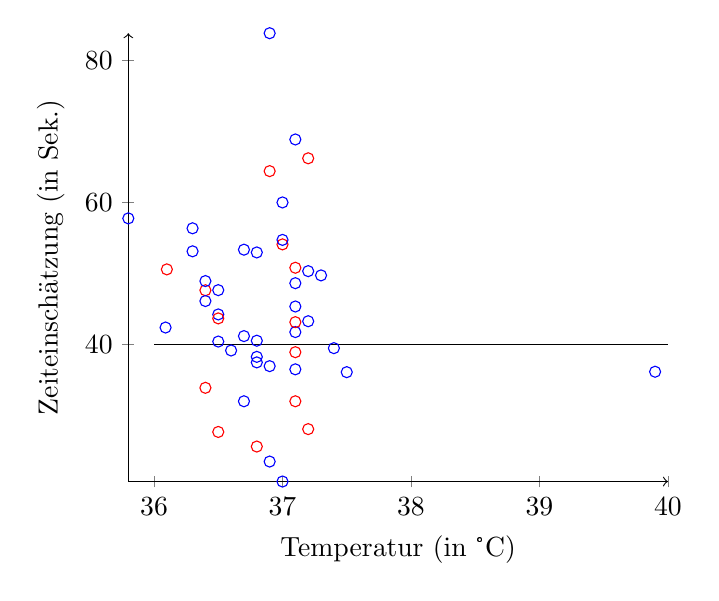
\begin{tikzpicture}
\begin{axis}[%
scatter/classes={%
    a={mark=o,draw=blue},
    b={mark=o,draw=red}},
    axis lines=middle,
    axis line style={->},
    x label style={at={(axis description cs:0.5,-0.1)},anchor=north},
    y label style={at={(axis description cs:-0.1,.5)},rotate=90,anchor=south},
    xlabel={Temperatur (in °C)},
    ylabel={Zeiteinschätzung (in Sek.)}]
     \addplot[domain=36:40]{39.9};
    \addplot[scatter,only marks,%
    scatter src=explicit symbolic]%
table[meta=label] {
x y label
35.8 57.75 a
36.09 42.34 a
36.1 50.55 b
36.3 53.1 a
36.3 56.35 a
36.4 47.6 b
36.4 46.08 a
36.4 48.9 a
36.4 33.83 b
36.5 27.6 b
36.5 44.19 a
36.5 43.63 b
36.5 40.36 a
36.5 47.62 a
36.6 39.1 a
36.7 53.33 a
36.7 41.13 a
36.7 31.93 a
36.8 40.48 a
36.8 52.94 a
36.8 25.54 b       
36.8 38.2 a
36.8 37.42 a
36.9 23.42 a
36.9 64.42 b
36.9 83.89 a
36.9 36.89 a
37.00 20.6 a
37.00 60 a
37.00 54.08  b
37.00 54.71 a
37.1 38.86 b
37.1 41.7 a
37.1 45.31 a
37.1 68.89 a
37.1 36.44 a
37.1 43.1 b
37.1 50.78 b
37.1 31.93 b
37.1 48.6 a
37.2 66.23 b
37.2 43.23 a
37.2 28 b
37.2 50.3 a
37.3 49.7 a
37.4 39.43 a
37.5 36.04 a
39.9 36.1 a
    };
\end{axis}
\end{tikzpicture}
\caption{Zeiteinschätzung von 40 Sekunden ohne Gespräch nach Temperatur}
\label{Zeit40sekTemp}
\end{minipage}
\hfill
\begin{minipage}[t]{0.49\linewidth}
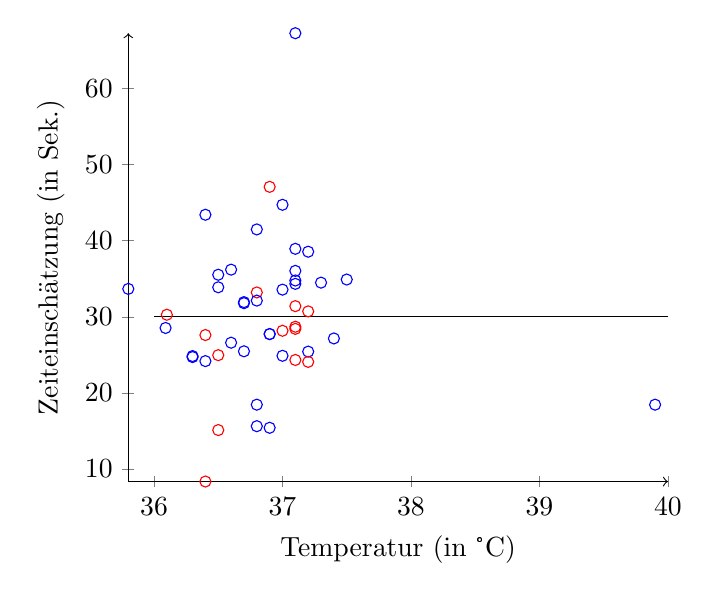
\begin{tikzpicture}
\begin{axis}[%
scatter/classes={%
    a={mark=o,draw=blue},
    b={mark=o,draw=red}},
    axis lines=middle,
    axis line style={->},
    x label style={at={(axis description cs:0.5,-0.1)},anchor=north},
    y label style={at={(axis description cs:-0.1,.5)},rotate=90,anchor=south},
    xlabel={Temperatur (in °C)},
    ylabel={Zeiteinschätzung (in Sek.)}]
    % Orientierungslinie
        \addplot[domain=36:40]{30};
        % Scatter
    \addplot[scatter,only marks,%
    scatter src=explicit symbolic]%
table[meta=label] {
x y label
35.8 33.67 a
36.09 28.53 a
36.1 30.27 b
36.3 24.70 a
36.3 24.83 a
36.4 27.60 b
36.4 43.42 a
36.4 24.17 a
36.4 8.33 b
36.5 15.1 b
36.5 33.88 a
36.5 24.95 b
36.5 35.53 a
36.6 36.2 a
36.6 26.59 a
36.7 31.79 a
36.7 31.93 a
36.7 25.46 a
36.8 41.49 a
36.8 15.61 a
36.8 33.2 b
36.8 18.44 a
36.8 32.13 a
36.9 27.72 a
36.9 47.09 b
36.9 27.73 a
36.9 15.40 a
37.00 44.73 a
37.00 33.57 a
37.00 28.16  b
37.00 24.87 a
37.1 28.69 b
37.1 34.33 a
37.1 34.77 a
37.1 36.04 a
37.1 38.94 a
37.1 28.41 b
37.1 24.32 b
37.1 31.4 b
37.1 67.30 a
37.2 30.71 b
37.2 25.42 a
37.2 24.07 b
37.2 38.56 a
37.3 34.49 a
37.4 27.15 a
37.5 34.9 a
39.9 18.44 a
        };
\end{axis}
\end{tikzpicture}
\caption{Zeiteinschätzung von 30 Sekunden ohne Gespräch nach Temperatur}
\label{Zeit30sekTemp}
\end{minipage}
\end{figure}

%%%%%%%%%%%%%%%%%%%%%%%%%%%%%%%%% HISTO TEMP %%%%%%%%%%%%%%%%%%%%%
\begin{figure}[H]
\begin{filecontents}{data.csv}
dist
  57.75
 42.34
 50.55
 53.1
 56.35
 47.6
 46.08
 48.9
 33.83
 27.6
 44.19
 43.63
 40.36
 47.62
 39.1
 53.33
 41.13
 31.93
 40.48
 52.94
25.54
 38.2
37.42
23.42
 64.42
 83.89
36.89
20.6
 60
 54.08 
 54.71
 38.86
 41.7
 45.31
 68.89
36.44
 43.1
50.78
31.93
48.6
66.23
 43.23
 28
 50.3
 49.7
 39.43
 36.04
36.1
\end{filecontents}
\begin{minipage}[t]{0.49\linewidth}
\begin{tikzpicture}
\begin{axis}[
    ybar,
    ymin=0
]
\addplot +[
    hist={
        bins=10,
        data min=0.5,
        data max=50
    }   
] table [y index=0] {data.csv};
\end{axis}
\end{tikzpicture}
\caption{Anzahl der Personen(y), welche die jeweilige Zeiteinschätzung(x) angaben - 40 Sekunden ohne Gespräch nach Temperatur.}
\label{HistZeit40sekTemp}
\end{minipage}
\hfill
\begin{filecontents}{data.csv}
dist
  33.67
 28.53
 30.27
 24.70
 24.83
 27.60
 43.42
 24.17
 8.33
 15.1
 33.88
 24.95
 35.53
 36.2
 26.59
 31.79
 31.93
 25.46
 41.49
 15.61
 33.2
 18.44
 32.13
 27.72
 47.09
 27.73
 15.40
 44.73
 33.57
 28.16 
 24.87
 28.69
 34.33
 34.77
 36.04
 38.94
 28.41
 24.32
 31.4
 67.30
 30.71
 25.42
 24.07
 38.56
 34.49
 27.15 
 34.9
18.44
\end{filecontents}
\begin{minipage}[t]{0.49\linewidth}
\begin{tikzpicture}
\begin{axis}[
    ybar,
    ymin=0
]
\addplot +[
    hist={
        bins=10,
        data min=0.5,
        data max=50
    }   
] table [y index=0] {data.csv};
\end{axis}
\end{tikzpicture}
\caption{Anzahl der Personen(y), welche die jeweilige Zeiteinschätzung(x) angaben - 30 Sekunden ohne Gespräch nach Temparatur.}
\label{HistZeit30sekTemp}
\end{minipage}
\end{figure}

%%%%%%%%%%%%%%%%%%%%%%%%%%%%%%%%%%%%%%%%%%%%%%%%%%%%%%%% HISTO TEMP %%%%%%

Lediglich eine Versuchsperson lag mit 39,9° C über der Durchschnittstemperatur(\textbf{durchschnittstemperatur x grad c}). Auffällig ist, dass es die meisten Abweichungen im direkten Umfeld von 37°C gab, bei niedrigerer Temperatur nähern sich die Zeiteinschätzungen dem Ergebnis etwas mehr an. Auch die Versuchsperson mit der sehr hohen Temperatur liegt in einer Schätzung nah am erwarteten Ergebnis.





%%%%%%%%%%%%%%%%%%%
\begin{figure}[H]
\begin{minipage}[t]{0.49\linewidth}
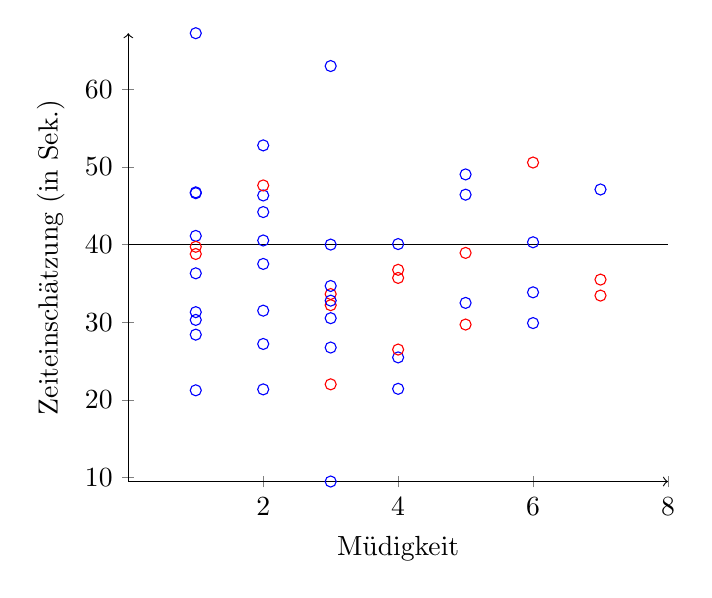
\begin{tikzpicture}
\begin{axis}[%
scatter/classes={%
    a={mark=o,draw=blue},
    b={mark=o,draw=red}},
    axis lines=middle,
    axis line style={->},
    x label style={at={(axis description cs:0.5,-0.1)},anchor=north},
    y label style={at={(axis description cs:-0.1,.5)},rotate=90,anchor=south},
    xlabel={Müdigkeit},
    ylabel={Zeiteinschätzung (in Sek.)}]
    \addplot[domain=0:8]{40};
    \addplot[scatter,only marks,%
    scatter src=explicit symbolic]%
table[meta=label] {
x y label
1 30.3 a
1 38.79 b
1 46.62 a
1 67.23 a
1 41.12 a
1 28.4 a
1 36.30 a
1 39.72 b
1 46.73 a
1 31.3 a
1 21.23 a
2 21.35 a
2 31.49 a
2 46.33 a
2 40.53 a
2 47.62 b
2 44.19 a
2 52.78 a
2 37.51 a
2 27.2 a
3 33.63 b
3 40.00 a
3 32.20 b
3 32.78 a
3 26.74 a
3 63.00 a
3 22 b
3 34.67 a
3 9.48 a
3 30.52 a
4 40.07 a
4 36.75 b
4 35.71 b
4 25.47 a
4 26.48 b
4 21.42 a
5 46.43 a
5 49.04 a
5 29.70 b
5 38.93 b
5 32.49 a
6 40.3 a
6 33.85 a
6 29.89 a
6 50.57 b
7 35.49 b
7 47.10 a
7 33.43 b
    };
\end{axis}
\end{tikzpicture}
\caption{Zeiteinschätzung von 40 Sekunden ohne Gespräch nach Müdigkeit}
\label{Zeit40sekMued}
\end{minipage}
\hfill
\begin{minipage}[t]{0.49\linewidth}
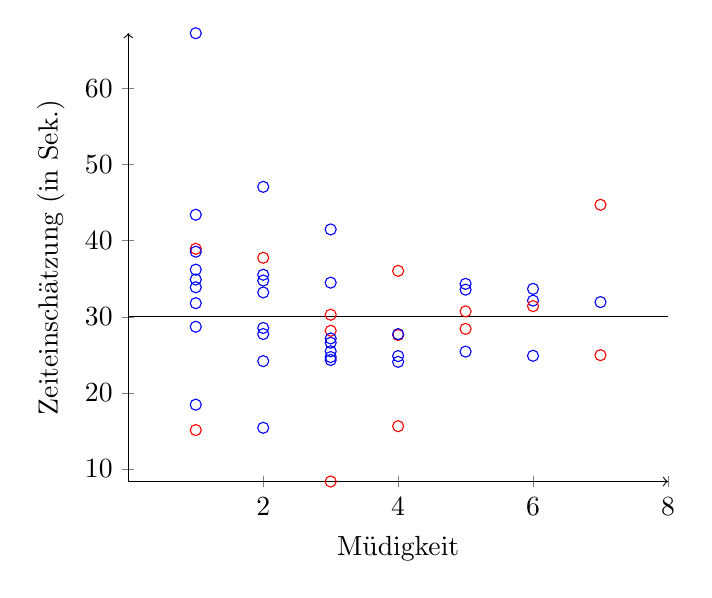
\begin{tikzpicture}
\begin{axis}[%
scatter/classes={%
    a={mark=o,draw=blue},
    b={mark=o,draw=red}},
    axis lines=middle,
    axis line style={->},
    x label style={at={(axis description cs:0.5,-0.1)},anchor=north},
    y label style={at={(axis description cs:-0.1,.5)},rotate=90,anchor=south},
    xlabel={Müdigkeit},
    ylabel={Zeiteinschätzung (in Sek.)}]
    % Orientierungslinie
        \addplot[domain=0:8]{30};
        % Scatter
    \addplot[scatter,only marks,%
    scatter src=explicit symbolic]%
table[meta=label] {
x y label
1 43.42 a
1 15.1 b
1 33.88 a
1 36.2 a
1 31.79 a
1 18.44 a
1 28.69 a
1 38.94 b
1 67.30 a
1 38.56 a
1 34.9 a
2 28.53 a
2 24.17 a
2 35.53 a
2 37.76 b
2 33.2 a
2 47.09 a
2 27.73 a
2 15.40 a
2 34.77 a
3 30.27 b
3 24.70 a
3 8.33 b
3 26.59 a
3 25.46 a
3 41.49 a
3 28.16 b
3 24.32 a
3 34.49 a
3 27.15 a
4 24.83 a
4 27.60 b
4 15.61 b
4 27.72 a
4 36.04 b
4 24.07 a
5 33.57 a
5 34.33 a
5 28.41 b
5 30.71 b
5 25.42 a
6 33.67 a
6 32.13 a
6 24.87 a
6 31.4 b
7 24.95 b
7 31.93 a
7 44.73 b
        };
\end{axis}
\end{tikzpicture}       
\caption{Zeiteinschätzung von 30 Sekunden ohne Gespräch nach Müdigkeit}
\label{Zeit30sekMued}
\end{minipage}
\end{figure}


%%%%%%%%%%%%%%%%%%%%%%%%%%%%%%%%% HISTO MÜDE %%%%%%%%%%%%%%%%%%%%%
\begin{figure}[H]
\begin{filecontents}{data.csv}
dist
   30.3
   38.79
 46.62
 67.23
 41.12
 28.4
 36.30
 39.72
 46.73
 31.3
 21.23
 21.35
 31.49
 46.33
 40.53
 47.62
 44.19
 52.78
 37.51
 27.2
 33.63
 40.00
 32.20
 32.78
 26.74
 63.00
 22
 34.67
 9.48
 30.52
 40.07
 36.75
 35.71
 25.47
 26.48
 21.42
 46.43
 49.04
 29.70
 38.93
 32.49
 40.3
 33.85
 29.89
 50.57
 35.49
 47.10
 33.43
\end{filecontents}
\begin{minipage}[t]{0.49\linewidth}
\begin{tikzpicture}
\begin{axis}[
    ybar,
    ymin=0
]
\addplot +[
    hist={
        bins=10,
        data min=0.5,
        data max=50
    }   
] table [y index=0] {data.csv};
\end{axis}
\end{tikzpicture}
\caption{Anzahl der Personen(y), welche die jeweilige Zeiteinschätzung(x) angaben - 40 Sekunden ohne Gespräch nach Müdigkeit.}
\label{HistZeit40sekMued}
\end{minipage}
\hfill
\begin{filecontents}{data.csv}
dist
  33.67
 28.53
 30.27
 24.70
 24.83
 27.60
 43.42
 24.17
 8.33
 15.1
 33.88
 24.95
 35.53
 36.2
 26.59
 31.79
 31.93
 25.46
 41.49
 15.61
 33.2
 18.44
 32.13
 27.72
 47.09
 27.73
 15.40
 44.73
 33.57
 28.16 
 24.87
 28.69
 34.33
 34.77
 36.04
 38.94
 28.41
 24.32
 31.4
 67.30
 30.71
 25.42
 24.07
 38.56
 34.49
 27.15 
 34.9
18.44
\end{filecontents}
\begin{minipage}[t]{0.49\linewidth}
\begin{tikzpicture}
\begin{axis}[
    ybar,
    ymin=0
]
\addplot +[
    hist={
        bins=10,
        data min=0.5,
        data max=50
    }   
] table [y index=0] {data.csv};
\end{axis}
\end{tikzpicture}
\caption{Anzahl der Personen(y), welche die jeweilige Zeiteinschätzung(x) angaben - 30 Sekunden ohne Gespräch nach Müdigkeit.}
\label{HistZeit30sekMued}
\end{minipage}
\end{figure}

%%%%%%%%%%%%%%%%%%%%%%%%%%%%%%%%%%%%%%%%%%%%%%%%%%%%%%%% HISTO MÜDE %%%%%%
%%%%%%%%%%%%%%%%%%%
%%%%%%%%%%%%%%%%%%%%%%%%%%%%%%%%%%%%%%%%%%%%%%%%%%%%%%%%%%%%%%%%%%%%%%%%%%%%%%%%%%%%%%%%%


Die Müdigkeitsskala erstreckt sich von 1 (nicht müde) bis 10 (sehr müde).\\
Die meisten Versuchspersonen gaben einen Wert $<=$ 5 an, haben aber nicht besser geschätzt als jene, die angaben, überdurchschnittlich müde zu sein. Auffällig ist hier, dass müdere Versuchspersonen in beiden Schätzungen insgesamt näher am erwarteten Wert liegen.

%%%% SCATTERPLOTS MIT GESRPÄCH
%%%%%%%%%%%%%%%%%%%%%%%%%%%%%%%%%%%%%%%%%%%%%%%%%%%%%%%%%%%%%%%%%%%%%%%%%%%%%%%%%%%%%%%%%
% SCATTERPLOT ALTER

%%%%%%%%%%%%%%%%%%%%%%%%%%%%%%%%% HISTO alter %%%%%%%%%%%%%%%%%%%%%
\begin{figure}[H]
\begin{minipage}[t]{0.49\linewidth}
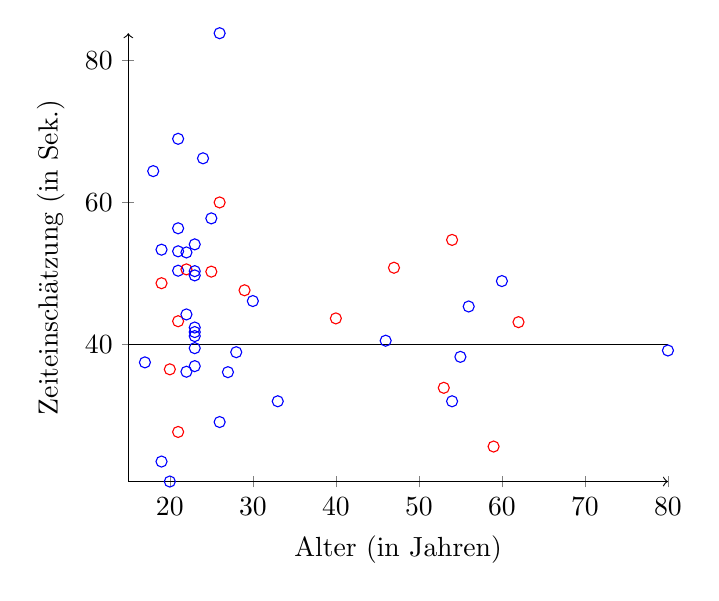
\begin{tikzpicture}
\begin{axis}[%
scatter/classes={%
    a={mark=o,draw=blue},
    b={mark=o,draw=red}},
    axis lines=middle,
    axis line style={->},
    x label style={at={(axis description cs:0.5,-0.1)},anchor=north},
    y label style={at={(axis description cs:-0.1,.5)},rotate=90,anchor=south},
    xlabel={Alter (in Jahren)},
    ylabel={Zeiteinschätzung (in Sek.)}]
    % Orientierungslinie
        \addplot[domain=15:80]{40};
        % Scatter
    \addplot[scatter,only marks,%
    scatter src=explicit symbolic]%
table[meta=label] {
x y label
17 37.42 a
18 64.42 a
19 53.33 a
19 23.42 a
19 48.6 b
20 20.6 a
20 36.44 b
21 53.1 a
21 56.35 a
21 27.6 b
21 50.36 a
21 68.98 a
21 43.23 b
22 50.55 b
22 44.19 a
22 52.94 a
22 36.1 a
23 54.08 a
23 42.34 a
23 41.13 a
23 36.89 a
23 41.7 a
23 50.3 a
23 49.7 a
23 39.43 a
24 66.23 a
25 50.23 b
25 57.75 a
26 60 b
26 83.89 a
26 29.00 a
27 36.04 a
28 38.86 a
29 47.6 b
30 46.08 a
33 31.93 a
40 43.63 b
46 40.48 a
47 50.78 b
53 33.83 b
54 54.71 b
54 31.93 a
55 38.2 a
56 45.31 a
59 25.54 b
60 48.9 a
62 43.1 b       
80 39.1 a
        };
\end{axis}
\end{tikzpicture}
\caption{Zeiteinschätzung von 40 Sekunden mit Gespräch nach Alter}
\label{Zeit40sekAltMitGespr}
\end{minipage}
\hfill
\begin{filecontents}{data.csv}
dist
 42.34
 41.13
 36.89
 41.7
 50.3
 49.7
 39.43
 66.23
 50.23
 57.75
 60
 83.89
 29.00
 36.04
 38.86
 47.6
 46.08
 31.93
 43.63
 40.48
 50.78
 33.83
 54.71
 31.93
 38.2
 45.31
 25.54
 48.9
 43.1       
 39.1
\end{filecontents}
\begin{minipage}[t]{0.49\linewidth}
\begin{tikzpicture}
\begin{axis}[
    ybar,
    ymin=0
]
\addplot +[
    hist={
        bins=10,
        data min=0.5,
        data max=50
    }   
] table [y index=0] {data.csv};
\end{axis}
\end{tikzpicture}
\caption{Anzahl der Personen(y), welche die jeweilige Zeiteinschätzung(x) angaben - 40 Sekunden mit Gespräch nach Alter.}
\label{Zeit40sekAlt}
\end{minipage}
\end{figure}

Es ist auffällig, dass viele der jüngeren Versuchspersonen die Zeit im Gespräch unterschätzten. Nichtsdestoweniger lagen aber auch viele der Versuchspersonen aus allen Altersklassen immernoch recht nah am erwarteten Wert.
%%%%%%%%%%%%%%%%%%%%%%%%%%%%%%%%%%%%%%%%%%%%%%%%%%%%%%%%%%%%%%%%%%%%%%%%%%%%%%%%%%
\begin{figure}[H]
\begin{minipage}[t]{0.49\linewidth}
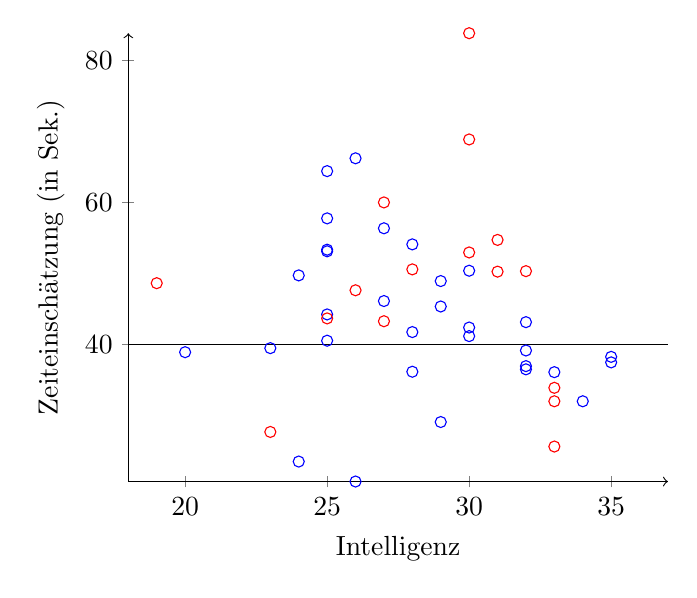
\begin{tikzpicture}
\begin{axis}[%
scatter/classes={%
    a={mark=o,draw=blue},
    b={mark=o,draw=red}},
    axis lines=middle,
    axis line style={->},
    x label style={at={(axis description cs:0.5,-0.1)},anchor=north},
    y label style={at={(axis description cs:-0.1,.5)},rotate=90,anchor=south},
    xlabel={Intelligenz},
    ylabel={Zeiteinschätzung (in Sek.)}]
  \addplot[domain=18:37]{40};
    \addplot[scatter,only marks,%
    scatter src=explicit symbolic]%
table[meta=label] {
x y label
19 48.6 b
20 38.86 a
23 27.6 b
23 39.43 a
24 23.42 a
24 49.7 a
25 64.42 a
25 53.33 a
25 53.1 a
25 44.19 a
25 57.75 a
25 43.63 b
25 40.48 a
26 20.6 a
26 66.23 a
26 47.6 b
27 56.35 a
27 43.23 b
27 60 b
27 46.08 a
28 50.55 b
28 36.1 a
28 54.08 a
28 41.7 a
29 29 a
29 45.31 a
29 48.9 a
30 50.36 a
30 68.89 b
30 52.94 b
30 42.34 a
30 41.13 a
30 83.89 b
31 54.71 b
31 50.23 b
32 36.44 a
32 36.89 a
32 50.3 b
32 43.1 a
32 39.1 a
33 36.04 a
33 31.93 b
33 25.54 b
33 33.83 b
34 31.93 a
35 38.2 a
35 37.42 a
        };
\end{axis}
\end{tikzpicture}
\caption{Zeiteinschätzung von 40 Sekunden mit Gespräch nach Intelligenz}
\label{Zeit40sekGesprInt}
\end{minipage}
\hfill
\begin{filecontents}{data.csv}
dist
  48.6
 38.86
 27.6
 39.43
 23.42
 49.7
 64.42
 53.33
 53.1
 44.19
 57.75
 43.63
 40.48
 20.6
 66.23
 47.6
 56.35
 43.23
 60
 46.08
 50.55
 36.1
 54.08
 41.7
 29
 45.31
 48.9
 50.36
 68.89
 52.94
 42.34
 41.13
 83.89
 54.71
 50.23
 36.44
 36.89
 50.3
 43.1
 39.1
 36.04
 31.93
 25.54
 33.83
 31.93
 38.2
 37.42
\end{filecontents}
\begin{minipage}[t]{0.49\linewidth}
\begin{tikzpicture}
\begin{axis}[
    ybar,
    ymin=0
]
\addplot +[
    hist={
        bins=10,
        data min=0.5,
        data max=50
    }   
] table [y index=0] {data.csv};
\end{axis}
\end{tikzpicture}
\caption{Anzahl der Personen(y), welche die jeweilige Zeiteinschätzung(x) angaben - 40 Sekunden mit Gespräch nach Intelligenz.}
\label{HistZeit40sekGesprInt}
\end{minipage}
\end{figure}

Viele der durchschnittlich intelligenten Versuchspersonen schätzen die tatsächlich verstrichene Zeit als kürzer ein, wohingegen jene mit niedrigerer und höherer Intelligenz näher am Idealwert liegen. Hierbei sei wieder angemerkt, dass die meisten Versuchspersonen im Mittelwert \textbf{genau angeben} liegen und nur eine Minderheit die Extreme auf beiden Seiten darstellen.

%%%%%%%%%%%%%%%%%%%%%%%%%%%%%%%%%%%%%%%%%%%%%%%%%%%%%%%%%%%%%%%%%%%%%%%%%%%%%%%%%%%%%
\begin{figure}[H]
\begin{minipage}[t]{0.49\linewidth}
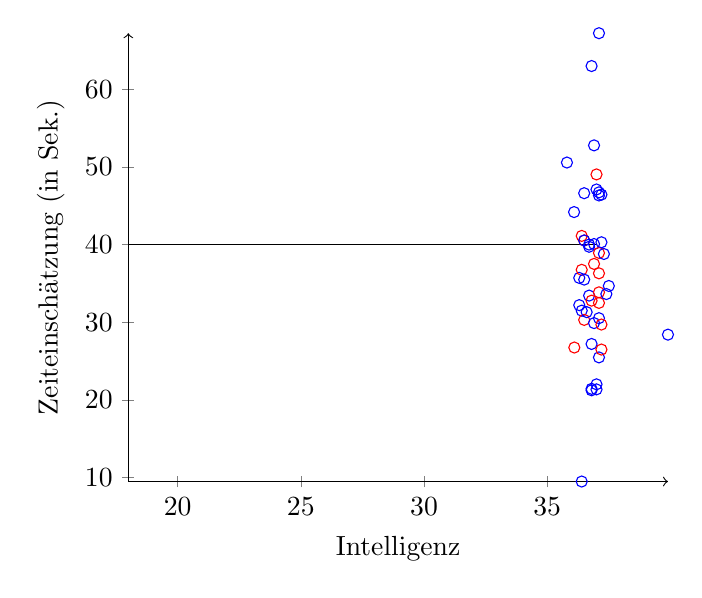
\begin{tikzpicture}
\begin{axis}[%
scatter/classes={%
    a={mark=o,draw=blue},
    b={mark=o,draw=red}},
    axis lines=middle,
    axis line style={->},
    x label style={at={(axis description cs:0.5,-0.1)},anchor=north},
    y label style={at={(axis description cs:-0.1,.5)},rotate=90,anchor=south},
    xlabel={Intelligenz},
    ylabel={Zeiteinschätzung (in Sek.)}]
  \addplot[domain=18:37]{40};
    \addplot[scatter,only marks,%
    scatter src=explicit symbolic]%
table[meta=label] {
x y label
35.8 50.57 a
36.09 44.19 a
36.1 26.74 b
36.3 32.2 a
36.3 35.71 a
36.4 41.12 b
36.4 31.49 a
36.4 9.48 a
36.4 36.75 b
36.5 30.3 b
36.5 46.62 a
36.5 40.53 b
36.5 40.53 a
36.5 35.49 a
36.6 31.3 a
36.7 39.72 a
36.7 40.00 a
36.7 33.43 a
36.8 21.23 a
36.8 27.2 a
36.8 32.78 b
36.8 63.00 a
36.8 21.42 a
36.9 52.78 a
36.9 37.51 b
36.9 40.07 a
36.9 29.89 a
37.00 21.35 a
37.00 22 a
37.00 49.04  b
37.00 47.1 a
37.1 36.3 b
37.1 46.73 a
37.1 46.33 a
37.1 30.52 a
37.1 25.47 a
37.1 38.93 b
37.1 32.49 b
37.1 33.85 b
37.1 67.23 a
37.2 26.48 b
37.2 46.43 a
37.2 29.7 b
37.2 40.3 a
37.3 38.79 a
37.4 33.63 a
37.5 34.67 a
39.9 28.4 a
        };
\end{axis}
\end{tikzpicture}
\caption{Zeiteinschätzung von 40 Sekunden mit Gespräch nach Temperatur}
\label{Zeit40sekGesprTemp}
\end{minipage}
\hfill
\begin{filecontents}{data.csv}
dist
   50.57
 44.19
 26.74
 32.2
 35.71
 41.12
 31.49
 9.48
 36.75
 30.3
 46.62
 40.53
 40.53
 35.49
 31.3
 39.72
 40.00
 33.43
 21.23
 27.2
 32.78
 63.00
 21.42
52.78
37.51
 40.07
 29.89
 21.35
 22
 49.04 
 47.1
 36.3
 46.73
 46.33
 30.52
 25.47
 38.93
32.49
 33.85
 67.23
 26.48
 46.43
 29.7
 40.3
 38.79
 33.63 
 34.67
28.4
\end{filecontents}
\begin{minipage}[t]{0.49\linewidth}
\begin{tikzpicture}
\begin{axis}[
    ybar,
    ymin=0
]
\addplot +[
    hist={
        bins=10,
        data min=0.5,
        data max=50
    }   
] table [y index=0] {data.csv};
\end{axis}
\end{tikzpicture}
\caption{Anzahl der Personen(y), welche die jeweilige Zeiteinschätzung(x) angaben - 40 Sekunden mit Gespräch nach Temperatur.}
\label{HistZeit40sekGesprTemp}
\end{minipage}
\end{figure}
Ähnlich wie bei den Einschätzungen ohne Gespräch befinden sich hier die stärksten Abweichungen bei den Versuchspersonen mit einer Temperatur knapp um 37°C. Bei Versuchspersonen mit niedrigerer Temperatur gibt es ebenfalls, wenn auch nicht so starke, Abweichungen.



%%%%%%%%%%%%%%%%%%%%%%%%%%%%%%%%%%%%%%%%%%%%%%%%%%%%%%%%%%%%%%%%%%%%%%%%%%%%%%%%%%%%%

\begin{figure}[H]
\begin{minipage}[t]{0.49\linewidth}
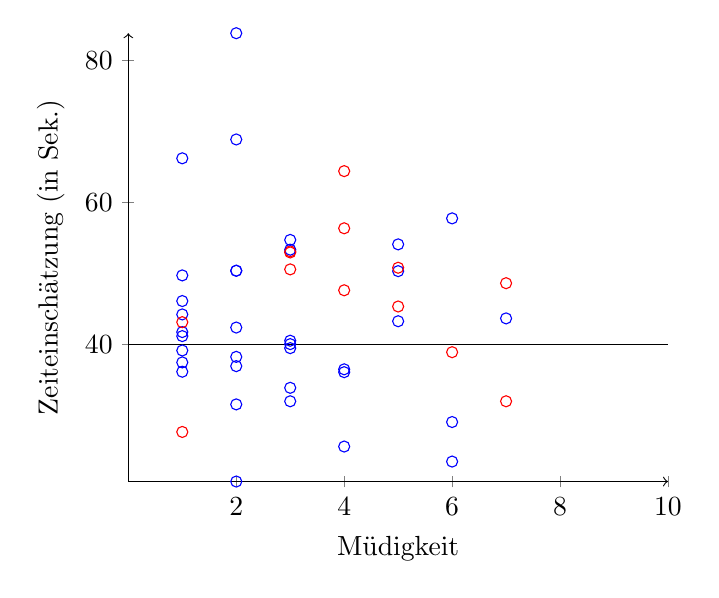
\begin{tikzpicture}
\begin{axis}[%
scatter/classes={%
    a={mark=o,draw=blue},
    b={mark=o,draw=red}},
    axis lines=middle,
    axis line style={->},
    x label style={at={(axis description cs:0.5,-0.1)},anchor=north},
    y label style={at={(axis description cs:-0.1,.5)},rotate=90,anchor=south},
    xlabel={Müdigkeit},
    ylabel={Zeiteinschätzung (in Sek.)}]
  \addplot[domain=0:10]{40};
    \addplot[scatter,only marks,%
    scatter src=explicit symbolic]%
table[meta=label] {
x y label
1 46.08 a
1 27.6 b
1 44.19 a
1 39.1 a
1 41.13 a
1 37.42 a
1 41.7 a
1 43.1 b
1 66.23 a
1 49.7 a
1 36.1 a
2 42.34 a
2 31.49 a
2 50.36 a
2 50.36 a
2 38.2 a
2 83.89 a
2 36.89 a
2 20.6 a
2 68.89 a
3 50.55 b
3 40.00 a
3 53.1 b
3 33.83 a
3 53.33 a
3 40.48 a
3 52.94 b
3 54.71 a
3 31.93 a
3 39.43 a
4 36.04 a
4 56.35 b
4 47.6 b
4 25.54 a
4 64.42 b
4 36.44 a
5 50.3 a
5 54.08 a
5 45.31 b
5 50.78 b
5 43.23 a
6 29.00 a
6 57.75 a
6 23.42 a
6 38.86 b
7 48.6 b
7 43.63 a
7 31.93 b
        };
\end{axis}
\end{tikzpicture}
\caption{Zeiteinschätzung von 40 Sekunden mit Gespräch nach Müdigkeit}
\label{Zeit40sekGesprMued}
\end{minipage}
\hfill
\begin{filecontents}{data.csv}
dist
 46.08
 27.6
 44.19
 39.1
 41.13
 37.42
 41.7
 43.1
 66.23
 49.7
 36.1
 42.34
 31.49
 50.36
 50.36
 38.2
 83.89
 36.89
 20.6
 68.89
 50.55
 40.00
 53.1
 33.83
 53.33
 40.48
 52.94
 54.71
 31.93
 39.43
 36.04
 56.35
 47.6
 25.54
 64.42
 36.44
 50.3
 54.08
 45.31
 50.78
 43.23
 29.00
 57.75
 23.42
 38.86
 48.6
 43.63
 31.93 
\end{filecontents}
\begin{minipage}[t]{0.49\linewidth}
\begin{tikzpicture}
\begin{axis}[
    ybar,
    ymin=0
]
\addplot +[
    hist={
        bins=10,
        data min=0.5,
        data max=50
    }   
] table [y index=0] {data.csv};
\end{axis}
\end{tikzpicture}
\caption{Anzahl der Personen(y), welche die jeweilige Zeiteinschätzung(x) angaben - 40 Sekunden mit Gespräch nach Müdigkeit.}
\label{HistZeit40sekMitGesprMued}
\end{minipage}
\end{figure}


Auffällig ist hier, dass die stärksten Abweichungen gerade bei den Personen liegen, die am wenigsten müde sind.

\subsection{Zeitschätzungen}
\begin{figure}[H]
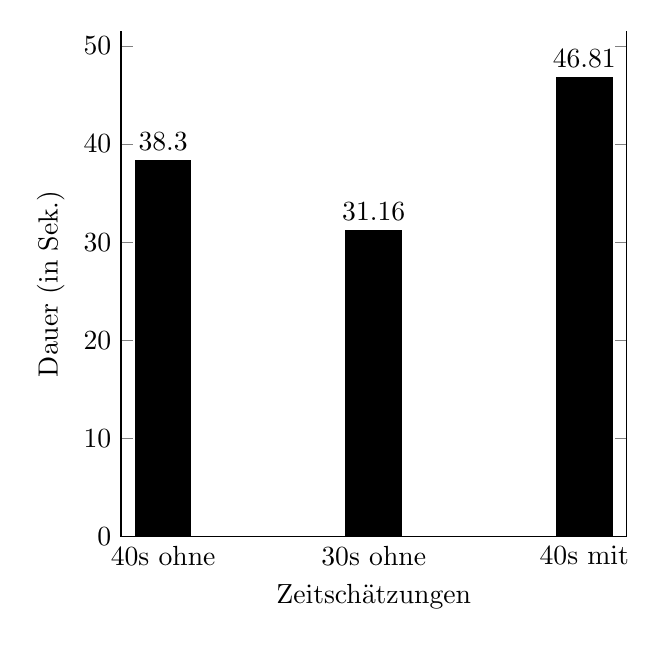
\begin{tikzpicture}
\begin{axis}[
     width  = 8cm,
     %hide y axis,
     axis x line*=bottom,
     height = 8cm,
     bar width=20pt,
     xlabel={Zeitschätzungen},
     ylabel={Dauer (in Sek.)},
     symbolic x coords={40s ohne,30s ohne,40s mit},
     nodes near coords,
     ymin=0,
     xtick=data
     ]
     
     \addplot[ybar, fill=black] coordinates {
          (40s ohne,38.30)
          (30s ohne,31.16)
          (40s mit,46.81)
         
     };
\end{axis}
\end{tikzpicture}
\caption{Gesamtheit aller Zeitschätzungen mit und ohne Gespräch}
\label{ZeitGespr}
\end{figure}



%Von links nach rechts sind dargestellt: die Einschätzungen von 40 Sekunden, dann 30 Sekunden und 40 Sekunden mit Gespräch als mögliche Beeinflussung. Auffällig ist, dass die dreißig Sekunden ziemlich genau getroffen wurden. Die Differenz zum Zielwert beträgt nicht einmal eine ganze Sekunde. Die vierzig Sekunden ohne das Gespräch, wurden durchschnittlich von den Versuchspersonen mit 36,41 um ca. vier Sekunden kürzer wahrgenommen. Die Variante mit dem Gespräch weist mit ca. 5 Sekunden Überschätzung der Zeit wie erwartet die größte Abweichung zum Zielwert auf, auch wenn sich dieser Differenzwert nicht sonderlich stark von dem des ersten Balken unterscheidet. Im Folgenden werden diese Werte separiert und als Versionen der Schätzungen vor und nach der VR dargelegt, um gegebenenfalls Einflüsse der VR ausfindig zu machen.
%%%%%%%%%%%%%%%%%%%%%%%%%%%%%%%%%%%%%%%%%%%%%%% vor der VR %%%%%%%%%%%%%%%%%%%%%%%%%%%%%%%
\begin{figure}[H]
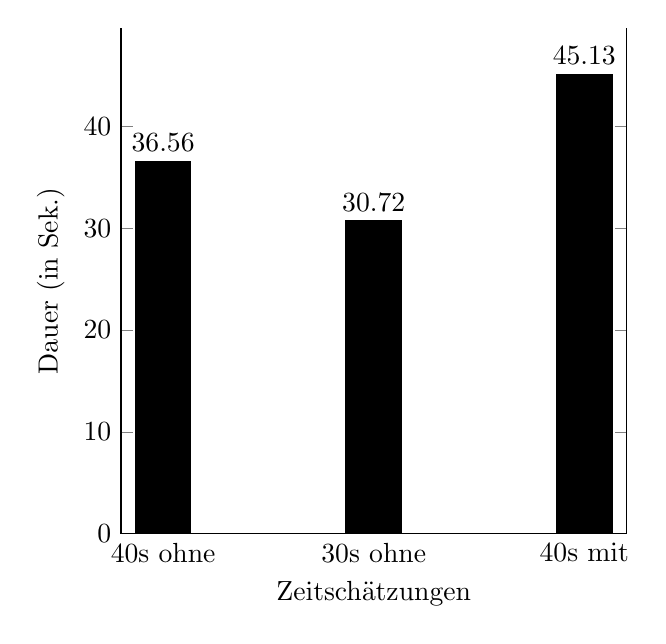
\begin{tikzpicture}
\begin{axis}[
     width  = 8cm,
     %hide y axis,
     axis x line*=bottom,
     height = 8cm,
     bar width=20pt,
     xlabel={Zeitschätzungen},
     ylabel={Dauer (in Sek.)},
     symbolic x coords={40s ohne,30s ohne,40s mit},
     nodes near coords,
     ymin=0,
     xtick=data
     ]
     
     \addplot[ybar, fill=black] coordinates {
          (40s ohne,36.56)
          (30s ohne,30.72)
          (40s mit,45.13)
         
     };
\end{axis}
\end{tikzpicture}
\caption{Zeitschätzung mit und ohne Gespräch vor der VR}
\label{ZeitVorVR}
\end{figure}

%Hier sind die Zeit-Einschätzungen vor der VR dargestellt.
%Die Schätzung der 30 Sekunden wird mit 30,72 Sekunden am präzisesten getroffen und die Zeitspanne der 40 Sekunden ohne Gespräch wird um ca. 3 Sekunden unterschätzt. Wieder schneidet die Schätzung mit dem Gespräch am schlechtesten ab. Die 40 Sekunden wurden um ca. 5 Sekunden länger geschätzt.
Die Durschnittswerte der Zeitabschätzungen der Versuchspersonen zeigen, dass es ihnen tendenziell leichter fiel, kürzere Zeiten (30 Sekunden) zu schätzen als längere (40 Sekunden) und die Abweichung der Schätzungen vom Zielwert hier geringer ausfällt.\\
Eine Versuchsperson hielt sich durchschnittlich 237,8 Sekunden in der VR-Welt auf, diese Zeit sollte er nach dem Experiment selbst abschätzen. Hier wäre es interessant zu erfahren, ob das Zeitempfinden sich, wie vermutet, wirklich beschleunigt hat, jedoch verhindern zu groß gewählte Zeitspannen (die kleinste betrug 0-7 Minuten) ein eindeutiges Ergebnis. Auf das betreffende Diagramm \ref{Spass} wird später noch Bezug genommen.
 

%%%%%%%%%%%%%%%%%%%%%%%%%%%%%%%%%%%%%%%%%%%%%%%%% nach der VR %%%%%%%%%%%%%%%%%%%%%%%%%%%%%%%
\begin{figure}[H]
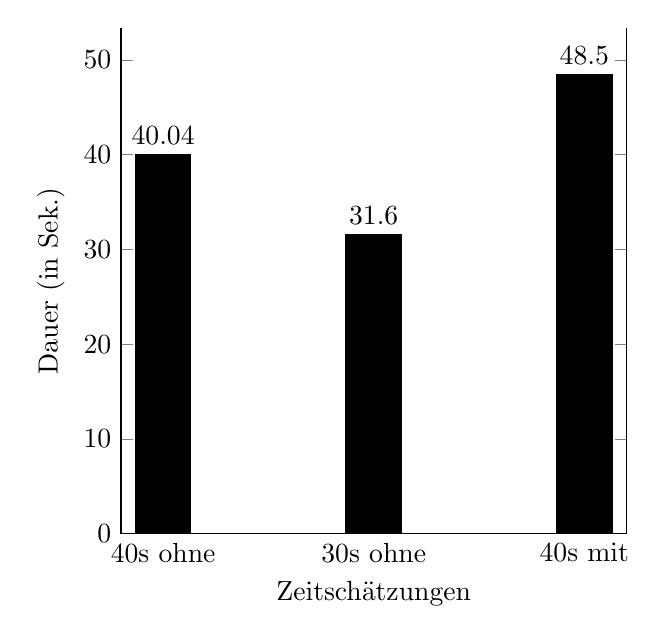
\begin{tikzpicture}
\begin{axis}[
     width  = 8cm,
     %hide y axis,
     axis x line*=bottom,
     height = 8cm,
     bar width=20pt,
     xlabel={Zeitschätzungen},
     ylabel={Dauer (in Sek.)},
     symbolic x coords={40s ohne,30s ohne,40s mit},
     nodes near coords,
     ymin=0,
     xtick=data
     ]
     
     \addplot[ybar, fill=black] coordinates {
          (40s ohne,40.04)
          (30s ohne,31.60)
          (40s mit,48.50)
         
     };
\end{axis}
\end{tikzpicture}
\caption{Zeitschätzung mit und ohne Gespräch nach der VR}
\label{ZeitNachVR}
\end{figure}

%Hier abgebildet sind die jeweiligen Zeit-Einschätzungen nach der VR.
%Die 40 Sekunden ohne das Gespräch werden mit durchschnittlichen 40,04 Sekunden am genauesten getroffen. Darauffolgend die 31,06 Sekunden, der 30 Sekunden Abschätzung und am schlechtesten schneidet wieder die 40 Sekunden Schätzung mit dem Gespräch ab. Hier wird die Zeit um 8,5 Sekunden überschätzt.
Im Vergleich der Schätzungs-Diagramme vor und nach dem VR-Aufenthalt ist zu erkennen, dass die Versuchspersonen die Zeit nach ihrem Aufenthalt in der VR-Welt stärker überschätzten als vor dem Aufenthalt (mit der Ausnahme der Schätzung von 40 Sekunden ohne Ablenkung). Während die 40 Sekunden ohne Ablenkung bei der zweiten Schätzung exakter ausfielen, entstand bei der Schätzung von 30 Sekunden ohne Ablenkung und der von 40 Sekunden mit Ablenkung eine Verschlechterung durch eine zu lange Einschätzung der Zeit.


%%%%%%%%%%%%%%%%%%%%%%%%%%%%%%%%%%%%%%%%%%%%%%%%%%%%%

\subsection{Einschätzung der vier Szenarien}

Die tatsächliche Dauer jedes Szenarios betrug achtzehn Sekunden.  \textbf{Tabelle 1} veranschaulicht je Szenario den dargestellten Inhalt, die Art des Zeitgebers und die Erwartung, ob die Zeitwahrnehmung dadurch entsprechend gedehnt oder verkürzt wird.
\begin{table}[H]

\centering
\begin{tabular}{llll}
        \hline
        \textbf{Szenario} & \textbf{Inhalt} & \textbf{Zeitgeber}& \textbf{Erwartungen} \\
        \hline
        a & LKW & a: schnelles Ticken & kürzer \\
        b & Vogel, Menschen & a: langsames Ticken & länger\\
        c & Park, Kind (rosa) & v: schnelles Schaukeln & kürzer\\
        d & Plakat, Kind (grün) & v: langsames Schaukeln & länger \\
        \hline
\end{tabular}
\caption{a=akustisch, v=visuell}

\label{AkVis}


\end{table}



\begin{figure}[H]
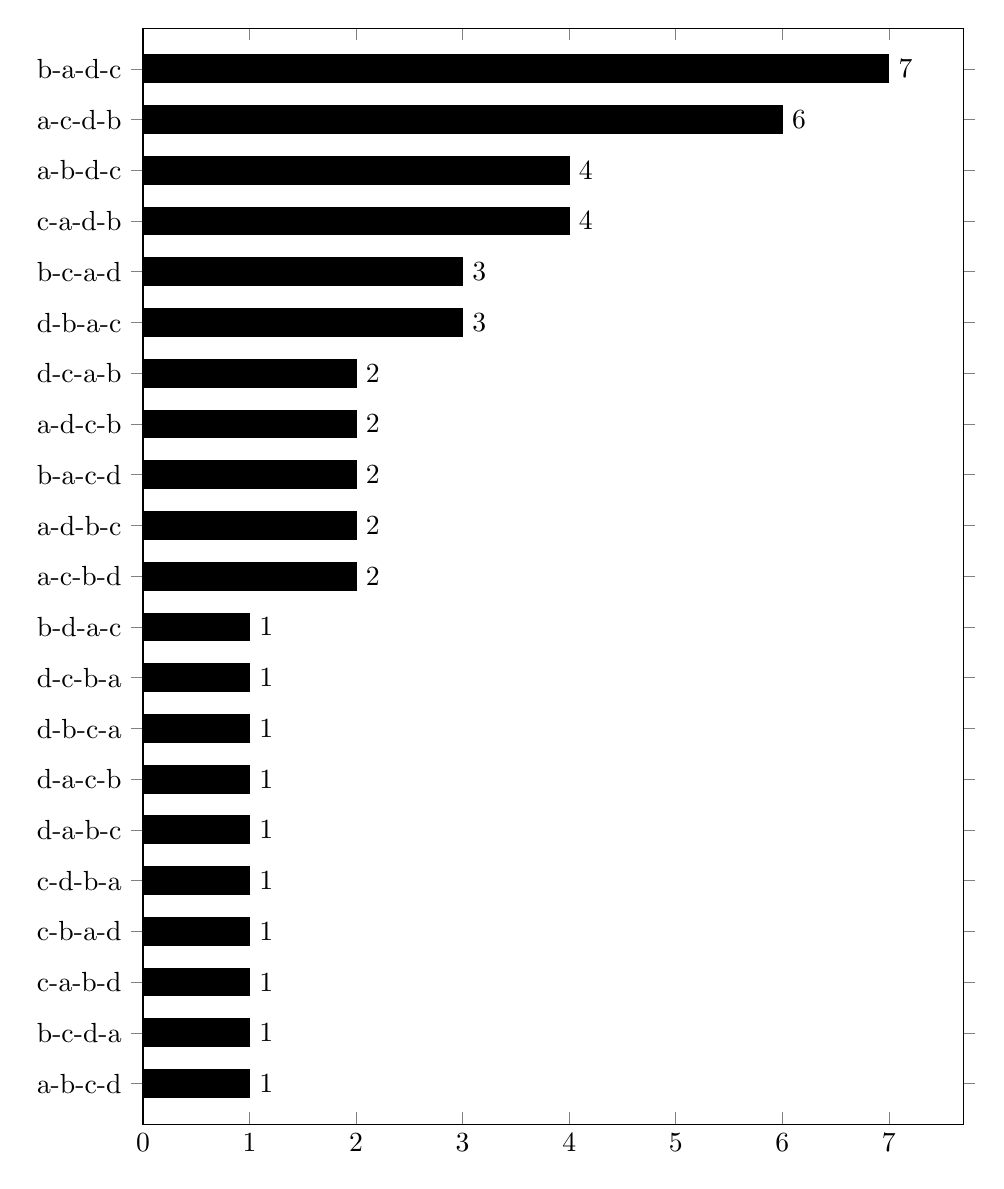
\begin{tikzpicture}
\begin{axis}[ xbar, xmin=0, width=12cm, height=15.5cm, enlarge y limits=0.04,
%xlabel={Probanden},
symbolic y coords={a-b-c-d,b-c-d-a,c-a-b-d,c-b-a-d,c-d-b-a,d-a-b-c,d-a-c-b,d-b-c-a,d-c-b-a,b-d-a-c,a-c-b-d,a-d-b-c,b-a-c-d,a-d-c-b,d-c-a-b,d-b-a-c,b-c-a-d,c-a-d-b,a-b-d-c,a-c-d-b,b-a-d-c},
ytick=data,
 nodes near coords,
  nodes near coords align={horizontal}, ]
 
 
\addplot[xbar, fill=black] coordinates {
(1,a-b-c-d)
(1,b-c-d-a)
(1,c-a-b-d)
(1,c-b-a-d)
(1,c-d-b-a)
(1,d-a-b-c)
(1,d-a-c-b)
(1,d-b-c-a)
(1,d-c-b-a)
(1,b-d-a-c)
(2,a-d-c-b)
(2,a-c-b-d)
(2,a-d-b-c)
(2,b-a-c-d)
(2,d-c-a-b)
(3,d-b-a-c)
(3,b-c-a-d)
(4,c-a-d-b)
(4,a-b-d-c)
(6,a-c-d-b)
(7,b-a-d-c)
};
 \end{axis}
  \end{tikzpicture}
  \caption{Szenarien von kurz nach lang}
  \label{SzenarienKurzLang}
  \end{figure}

Oben zu sehen: die Anzahl der Versuchspersonen, die die Szenarien entsprechend von kurz nach lang sortiert haben. D.h. konkret, dass insgesamt sieben Versuchspersonen   \textbf{b} für das kürzeste Szenario hielten und dann aufsteigend über \textbf{a} und \textbf{d} nach  \textbf{c} sortiert haben. \\
Sechs Versuchspersonen waren der Ansicht, \textbf{a} sei das kürzeste Szenario gewesen, gefolgt von \textbf{c}, \textbf{d} und schließlich \textbf{b}.\\

Die geschätzte Länge der Szenarien kann man nach visuellen und akustischen Zeitgebern trennen:

       
\begin{figure}[H]
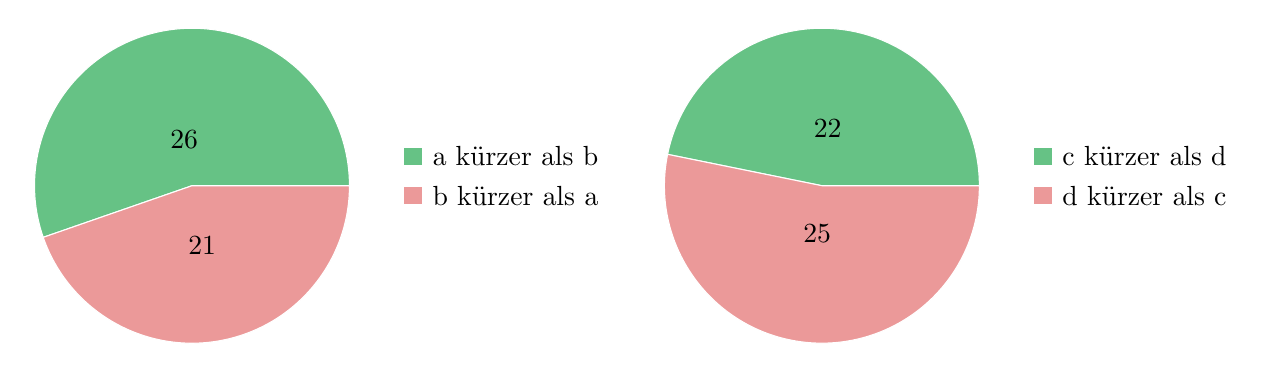
\begin{tikzpicture}
\tikzset{lines/.style={draw=white},}
\pie[color={greenOfApproval!60, redOfDisapproval!40},radius = 2 ,sum=auto, after number=,text=legend,every only number node/.style={text=black},style={lines}]{26/a kürzer als b,21/b kürzer als a}
\tikzset{lines/.style={draw=white},}
\pie[pos={8,0},radius = 2, color={greenOfApproval!60, redOfDisapproval!40},sum=auto, after number=,text=legend,every only number node/.style={text=black},style={lines}]{22/c kürzer als d,25/d kürzer als c}
\end{tikzpicture}
\caption{Links: Länge der akustischen Szenarien. Rechts: Länge der visuellen Szenarien}
\label{SzenarienVisuellAkustisch}
\end{figure} %[H]
       
        Die Tortendiagramme aus Abbildung 15 zeigen die beiden akustischen Szenarien \textbf{a} und \textbf{b} (links) und die visuellen Szenarien \textbf{c} und \textbf{d} jeweils in Relation zueinander. Hier sei nochmal erwähnt, dass jeweils die Szenarien \textbf{a} und \textbf{c} die kürzeren waren.\\
Durch die akustischen Zeitgeber haben 26 Versuchspersonen das Szenario \textbf{a} kürzer eingeschätzt als Szenario \textbf{b}. 21 Versuchspersonen waren gegenteiliger Meinung. Bei den visuellen Zeitgebern gibt es eine weniger eindeutige Meinung und das tatsächlich kürzere Szenario \textbf{c} haben 22 Personen erkannt, 25 schätzten \textbf{d} als kürzer ein.
       
       
Aus diesen Daten kann man herleiten, wie viele Personen ein Szenario als das kürzeste (Diagramm in gelb) bzw. längste (Diagramm in lila) empfunden haben.

\begin{figure}[ht]
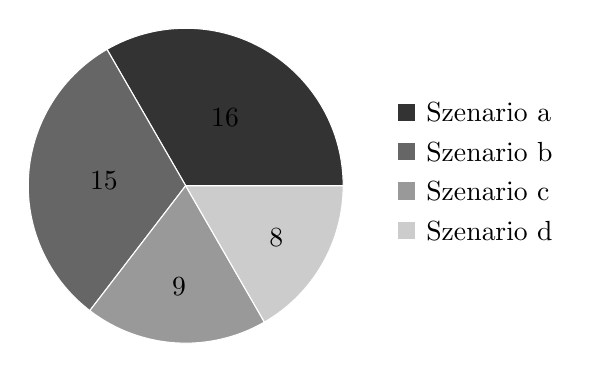
\begin{tikzpicture}
\tikzset{lines/.style={draw=white},}
\pie[color={yellowOfBrevity!80, yellowOfBrevity!60, yellowOfBrevity!40, yellowOfBrevity!20},radius = 2 ,sum=auto, after number=,text=legend,every only number node/.style={text=black},style={lines}]{16/Szenario a,15/Szenario b,9/Szenario c, 8/Szenario d}
\end{tikzpicture}
\caption{Welches Szenario war das kürzeste?}
\label{SzenarienKurz}
\end{figure}
       
Von allen Versuchspersonen haben 15 angegeben Szenario \textbf{a} als das kürzeste empfunden zu haben, knapp dahinter steht Szenario \textbf{b} mit 14 Stimmen. Im Vergleich dazu sind die Szenarien \textbf{c} und \textbf{d} mit 9 und 8 Stimmen etwas abgeschlagen. Eine eindeutige Mehrheit gibt es dennoch nicht.\\
Gleichermaßen kann man feststellen, welches Szenario von den meisten Personen als das längste bewertet wurde:

\begin{figure}[ht]
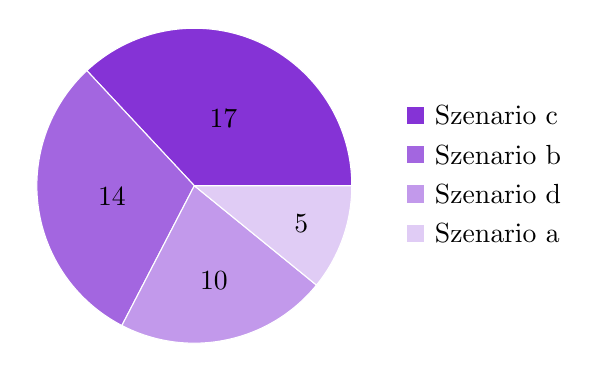
\begin{tikzpicture}
\tikzset{lines/.style={draw=white},}
\pie[color={purpleOfLengthiness!80, purpleOfLengthiness!60, purpleOfLengthiness!40, purpleOfLengthiness!20},radius = 2 ,sum=auto, after number=,text=legend,every only number node/.style={text=black},style={lines}]{17/Szenario c,14/Szenario b,10/Szenario d, 5/Szenario a}
\end{tikzpicture}
\caption{Welches Szenario war das längste?}
\label{SzenarienLang}
\end{figure}       

Auch bei der Bewertung des \textit{längsten} Szenarios gibt es keine ganz klare Mehrheit, dennoch heben sich zwei Szenarien etwas ab. 17 Versuchspersonen sind der Meinung, Szenario \textbf{c} sei das längste gewesen, danach kommen die Szenarien \textbf{b} mit 14 Stimmen und \textbf{d} mit 10 Stimmen. Abgeschlagen zum Schluss wird Szenario \textbf{a} mit nur 5 Stimmen genannt.\\
Auffällig ist, dass es keine einheitliche Meinung gibt, welches Szenario das längste oder kürzeste ist, allerdings zeichnen sich ein paar Tendenzen ab. So ist sich die relative Mehrheit der Versuchspersonen sicher, \textbf{a} sei das längste Szenario und dementsprechend wenige behaupten das direkte Gegenteil. Ähnlich verhält es sich bei Szenario \textbf{c}, welches auch verhältnismäßig oft als das längste bewertet wurde und nur sehr wenig als das kürzeste.\\
Auffällig ist allerdings auch, dass die Meinungen bei \textbf{b} recht stark auseinandergehen. Ein Großteil der Befragten sieht dieses Szenario entweder als das längste oder als das kürzeste an, es gibt nur wenig Verteilung im Mittelbereich.
Von Abb. \ref{SzenarienKurzLang} lassen sich keine Rückschlüsse auf die zuvor festgelegten Hypothesen oder die am Anfang des Experiments von der Versuchsperson erfragten Variablen schließen. Aufgrund dessen werden die Szenarien wie in Abbildung \ref{SzenarienVisuellAkustisch}
nach den Faktoren visuell und akustisch getrennt. Nahezu die Hälfte aller Versuchspersonen haben die "`schnellen'' Szenarien wirklich als schneller wahrgenommen. Dabei ist auffällig, dass bei den akustischen Szenarien 55,3\% der Personen \textbf{a} tatsächlich als schneller eingestuft haben. Bei den visuellen Szenarien wurde das "`schnelle'' Szenario \textbf{c} allerdings nur zu 46,8\% erkannt und damit als langsam angesehen. Daraus kann geschlussfolgert werden, dass es sich bei den akustischen Zeitgebern um die effektiveren handelt, die den Versuchspersonen im Vergleich zu den visuellen Szenarios erfolgreicher beeinflusst haben.\\
Die Hypothese, dass das Zeitgefühl durch schnelle Zeitgeber so beeinflusst
wird, dass die Zeit für die Versuchspersonen gefühlt schneller vergeht, lässt sich anhand Abb. \ref{LaengeSzenarien}) eindeutig für die "`schnelleren'' Szenarien bestätigen. Der geschätzte Durchschnittswert liegt für letztere jeweils deutlich unter der
tatsächlichen Länge von 18 Sekunden. Das Ergebnis der langsamen Szenarien \textbf{b} und
\textbf{d} unterscheidet sich zwar stark von den Ergebnissen der schnellen
Szenarien und zeigt, dass diese eindeutig länger eingeschätzt wurden, allerdings
entsprechen sie nicht der zu Beginn festgelegten zweiten Hypothese: Die Zeit vergeht
gefühlt langsamer, wenn eine Person durch einen langsamen Zeitgeber beeinflusst wird. Die
tatsächliche Länge von 18 Sekunden wurde somit deutlich verfehlt, allerdings zeigt es dennoch
die unterschiedliche Wirkungen von den schnellen und langsamen Zeitgebern, auch wenn es keinen
deutlichen Unterschied zwischen den beiden Arten der Zeitgeber gibt.
       
       
        %%%%%%%%%% DURCHSCHNITTZEITEN DER SZENARIEN
\begin{figure}        [H]
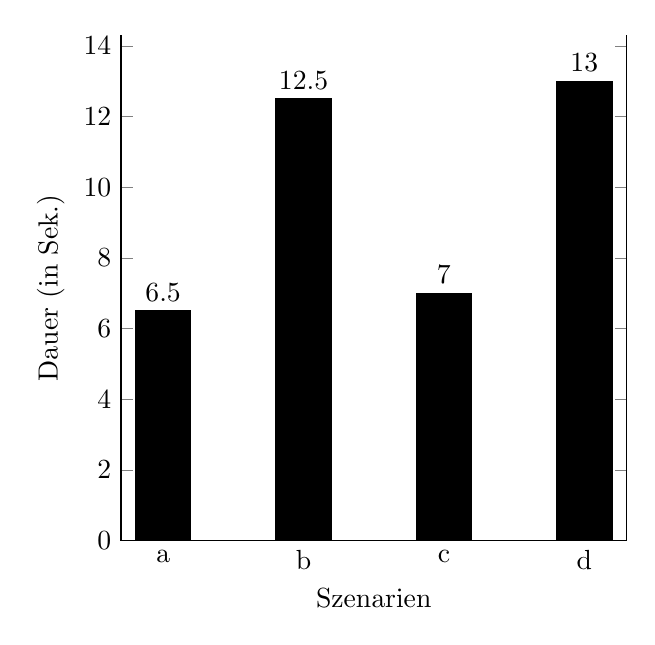
\begin{tikzpicture}
\begin{axis}[
     width  = 8cm,
     %hide y axis,
     axis x line*=bottom,
     height = 8cm,
     bar width=20pt,
     symbolic x coords={a,b,c,d},
     xlabel={Szenarien},
     ylabel={Dauer (in Sek.)},
     nodes near coords,
     ymin=0,
     xtick=data
     ]
     
     \addplot[ybar, fill=black] coordinates {
          (a,6.5)
          (b,12.5)
          (c,7)
          (d,13)
     };
\end{axis}
\end{tikzpicture}
\caption{Durchschnittlich geschätzte Längen der Szenarien}
\label{LaengeSzenarien}
\end{figure}

Die zeitlichen Einschätzungen bezüglich der Längen der einzelnen Szenarien sind als ermittelte Durchschnittswerte im obigen Balkendiagramm je Szenario dargestellt. Hier zu erkennen ist nun, dass das Szenario \textbf{d} mit durchschnittlichen 13 Sekunden als das Längste eingeschätzt wurde. Knapp dahinter liegt \textbf{b} mit 12,5 Sekunden, gefolgt von \textbf{a} mit 6,5 und \textbf{c} mit 7 Sekunden durchschnittlicher Schätzung.
%Interessant ist, dass eine Differenz von 0,5 Sekunden sowohl zwischen \textbf{a} und \textbf{c}, als auch \textbf{b} und \textbf{d} zu finden ist. Außerdem werden \textbf{b} und \textbf{d} nahezu doppelt solang geschätzt wie \textbf{a} und \textbf{c}.

\subsection{Beziehung zwischen Spaß- und Zeitempfinden}
Ein Faktor der die Zeitwahrnehmung beeinflusst haben könnte, ist hinsichtlich des Forschungspapiers "'Kinder, wie die Zeit vergeht!"'
\textit{Über Paradoxien in der Zeitwahrnehmung von Katja Irle} \cite{Irle2017} der Spaß am Geschehen.
Hierzu unsere Ergebnisse:
       
\begin{figure}[H]
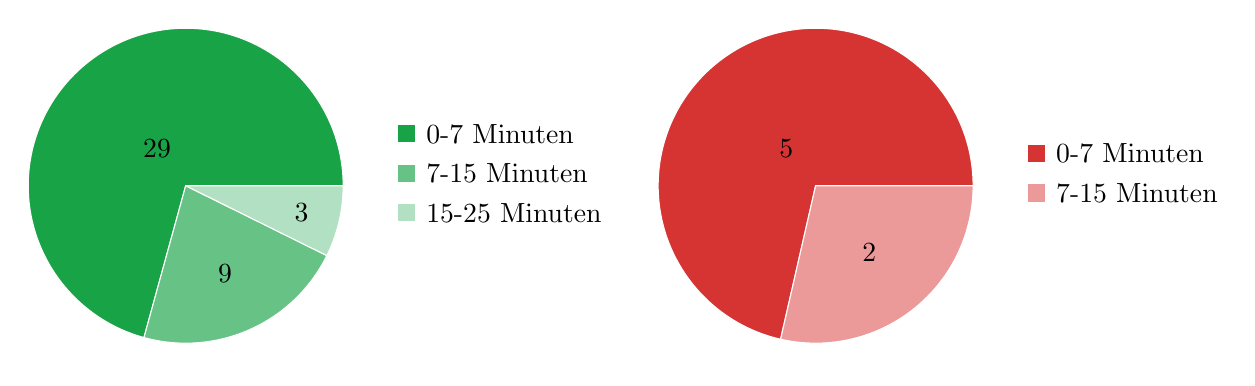
\begin{tikzpicture}
\tikzset{lines/.style={draw=white},}
\pie[color={greenOfApproval!90, greenOfApproval!60, greenOfApproval!30},radius = 2 ,sum=auto, after number=,text=legend,every only number node/.style={text=black},style={lines}]{29/0-7 Minuten,9/7-15 Minuten,3/15-25 Minuten}


\tikzset{lines/.style={draw=white},}
\pie[pos={8,0},radius = 2, color={redOfDisapproval!80, redOfDisapproval!40},sum=auto, after number=,text=legend,every only number node/.style={text=black},style={lines}]{5/0-7 Minuten,2/7-15 Minuten}
\end{tikzpicture}
\caption{Links: Spaß. Rechts: \textit{kein} Spaß}
\label{Spass}
\end{figure} %[H]

Die obigen beiden Tortendiagramme stellen unsere Versuchspersonen separiert dar. Links die Gruppe derer die Spaß an ihrem VR-Aufenthalt hatten und rechts die Versuchspersonen die angaben, dass sie keinen Spaß hatten. Innerhalb dieser Gruppen sind die Zeitschätzungen des VR-Aufenthalts abgebildet.Von den 41 Versuchspersonen die Spaß hatten, hat eine klare Mehrheit von 29 Personen geschätzt, dass die Dauer ihres VR-Aufenthalts im Intervall von 0-7 Minuten liegt. Weitere 9 Personen wählten die Zeitspanne von 7-15 Minuten und lediglich 3 schätzten die Dauer länger als 15 Minuten. Im rechten Tortendiagramm sind 7 Personen abgebildet, davon hat wieder die Mehrheit geschätzt, dass sie bis zu 7 Minuten in der VR waren und die restlichen 2 wählten das Intervall von 7-15 Minuten. Insgesamt entschieden sich also ca. 70\% von den insgesamt 48 Versuchspersonen für eine Zeitspanne von bis zu 7 Minuten. Was sich durch die im Rahmen haltende Größe unserer Welt und der Geschwindigkeit mit der man sich darin bewegen kann, eigentlich auch hätte erahnen lassen können.

Da die Intervalle zur Zeiteinschätzung des Aufenthalts in der VR von uns ungünstig gewählt wurden (Verbesserungsvorschläge hierzu, siehe in der Methodenkritik des Fazits), beziehen wir uns im Folgenden nur noch auf die tatsächliche Dauer, die von uns während der Versuchsdurchführung aufgenommen wurde.

Nach dem Aufenthalt der Versuchsperson in der VR-Welt wurden diese nach ihrem Spaßempfinden befragt. Das mit den Diagrammen dargestellte Ergebnis kann damit erklärt werden, dass die bereits gewählten Zeitspannen letztendlich nicht mehr auf unser Experiment, das zwischenzeitlich noch stark verändert wurde, passten. Geschickter wären kleinere Zeitspannen (0-2 Minuten, 3-4 Minuten,...) gewesen.\\
Unsere Hypothese vor dem Experiment war es, dass das Zeitempfinden durch das Spaßempfinden in der VR-Welt beeinflusst wird. Zu diesem Schluss ist auch der Psychologe Helmut Prior gekommen: "`Momente, in denen wir extrem angespannt oder aufgeregt sind, bleiben eher in der Erinnerung und kommen uns hinterher tendenziell lang vor.'' \cite{Irle2017} \\
Diese Hypothese lässt sich durch unsere Ergebnisse nicht belegen, da der Anteil der Versuchspersonen mit und ohne Spaß während ihres VR-Aufenthalts, die die Dauer im korrekten Zeitfenster geschätzt haben, jeweils bei gerundet 71 Prozent liegt. Dies ist ein weiterer Anhaltspunkt für die bereits erwähnten unpassend gewählten Zeitspannen.\\
Somit lassen sich keine Resultate aus den oben dargestellten Ergebnissen ziehen.

        \begin{figure}[H]
        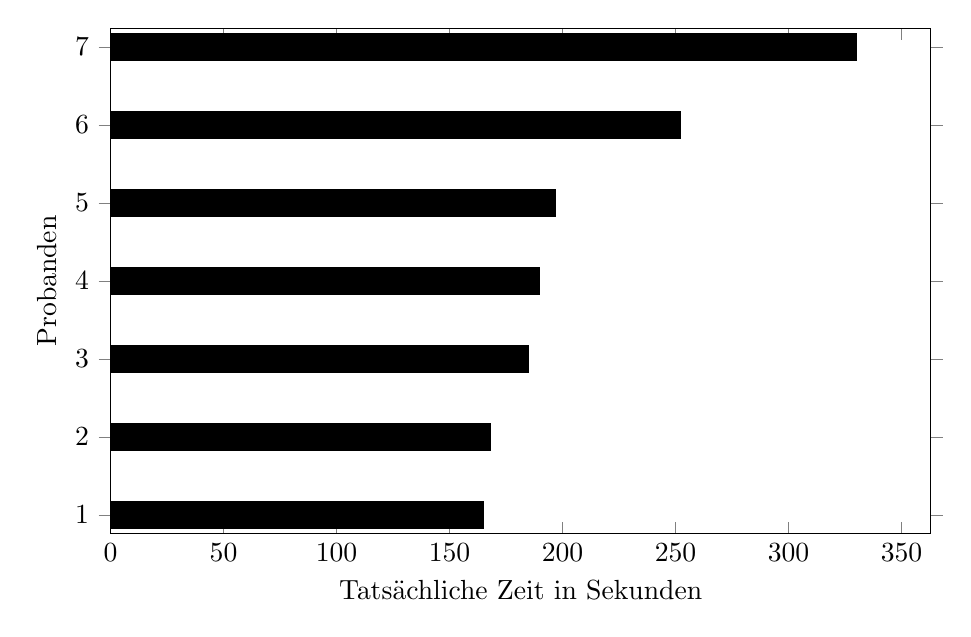
\begin{tikzpicture}
\begin{axis}[ xbar, xmin=0, width=12cm, height=8cm, enlarge y limits=0.04,
xlabel={Tatsächliche Zeit in Sekunden},ylabel={Probanden},
symbolic y coords={1,2,3,4,5,6,7},
ytick=data,
% nodes near coords,
 % nodes near coords align={horizontal},
 ]
 
\addplot[xbar, fill=black] coordinates {
(165,1)
(168,2)
(185,3)
(190,4)
(197,5)
(252,6)
(330,7)
};
 \end{axis}
  \end{tikzpicture}
  \caption{Tatsächliche Zeit der Versuchspersonen, die keinen Spaß hatten}
  \label{ZeitKeinSpass}
  %DURCHSCHNITT: 212,42 sek
        \end{figure}
In diesem Balkendiagramm wird die von uns aufgenommene tatsächliche Dauer des VR-Aufenthalts der sieben Versuchspersonen dargestellt, die nach eigener Angabe keinen Spaß an der Durchführung hatten. Das Minimum beträgt hier 165 Sekunden, also 2,75 Minuten, das Maximum beträgt 330 Sekunden, das sind 5,50 Minuten und der Median entspricht 190 Sekunden, also 3,16 Minuten. Die ersten fünf Zeiten liegen verhältnismäßig nah beieinander. Die unteren beiden Balken betrachtend, hielten sich die betreffenden Versuchspersonen länger in der VR auf.


                \begin{figure}[H]
        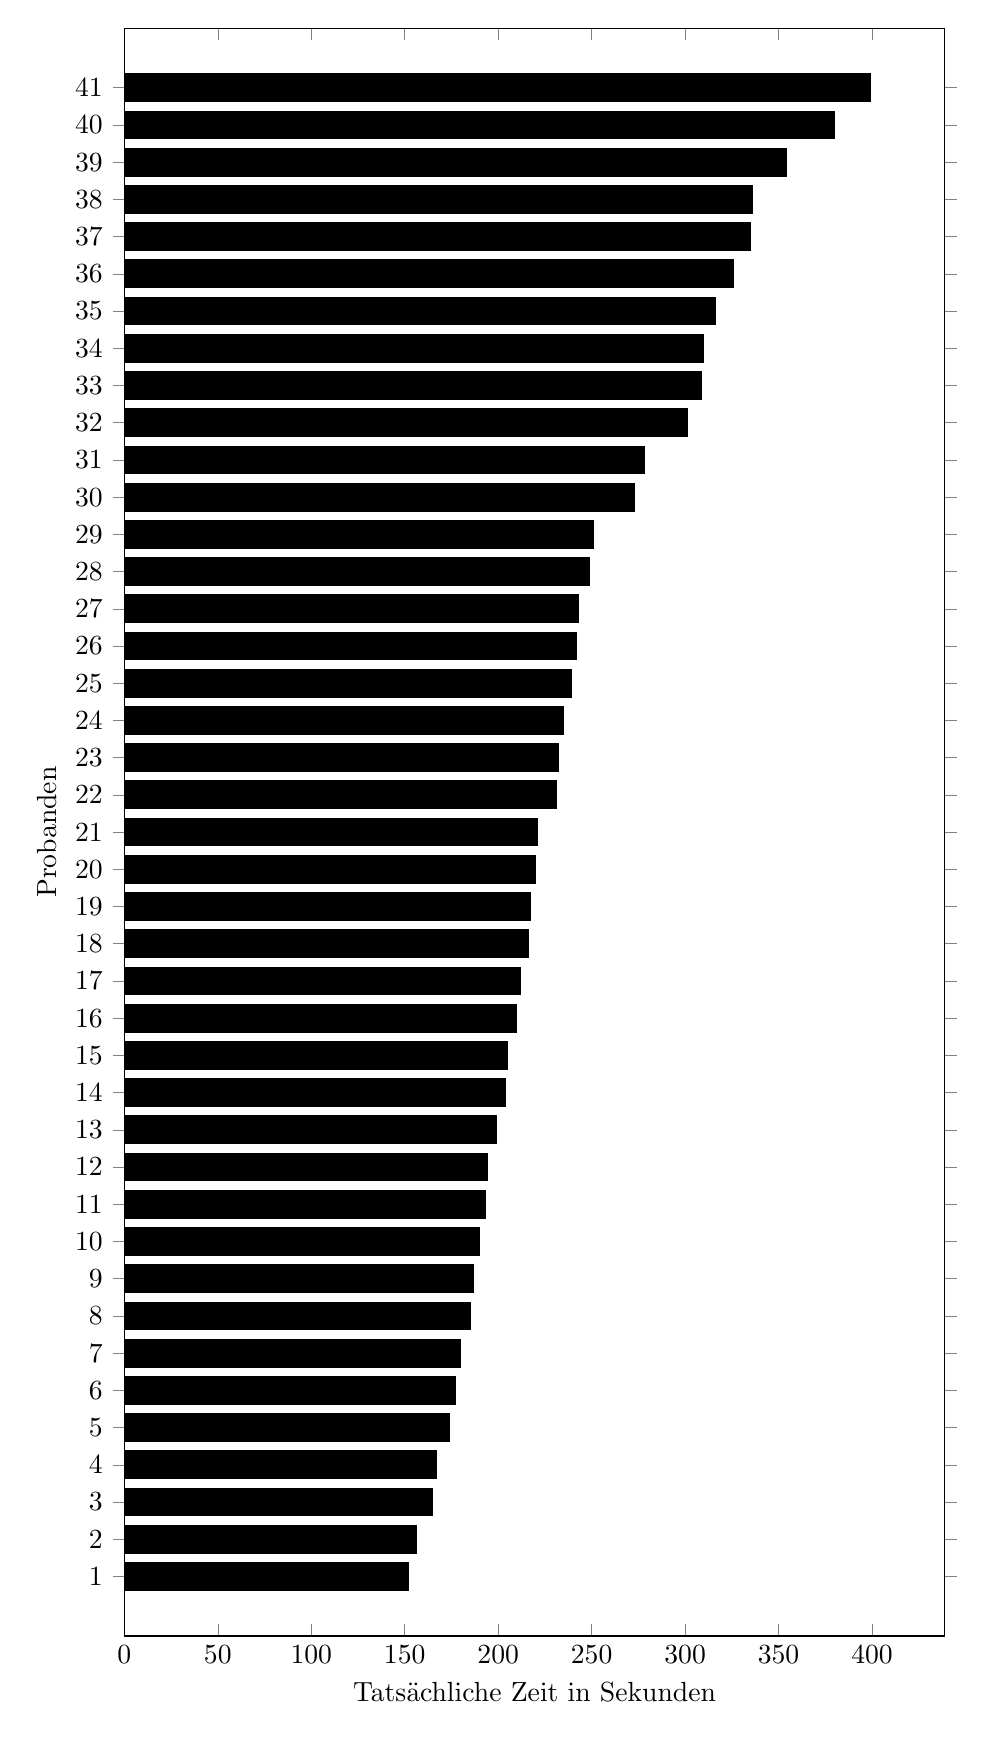
\begin{tikzpicture}
\begin{axis}[ xbar, xmin=0, width=12cm, height=22cm, enlarge y limits=0.04,
xlabel={Tatsächliche Zeit in Sekunden},
ylabel={Probanden},
symbolic y coords={1,2,3,4,5,6,7,8,9,10,11,12,13,14,15,16,17,18,19,20,21,22,23,24,25,26,27,28,29,30,31,32,33,34,35,36,37,38,39,40,41},
ytick=data,
% nodes near coords,
 % nodes near coords align={horizontal},
 ]
 
\addplot[xbar, fill=black] coordinates {
(152,1)
(156,2)
(165,3)
(167,4)
(174,5)
(177,6)
(180,7)
(185,8)
(187,9)
(190,10)
(193,11)
(194,12)
(199,13)
(204,14)
(205,15)
(210,16)
(212,17)
(216,18)
(217,19)
(220,20)
(221,21)
(231,22)
(232,23)
(235,24)
(239,25)
(242,26)
(243,27)
(249,28)
(251,29)
(273,30)
(278,31)
(301,32)
(309,33)
(310,34)
(316,35)
(326,36)
(335,37)
(336,38)
(354,39)
(380,40)
(399,41)
};
 \end{axis}
  \end{tikzpicture}
  \caption{Tatsächliche Zeit der Versuchspersonen, die Spaß hatten}
  \label{ZeitSpass}
  %DURCHSCHNITT: 240,56s
        \end{figure}
        Analog zum vorherigen Balkendiagramm werden hier auch die tatsächlichen Zeiten der VR-Aufenthalte veranschaulicht, nur mit dem Unterschied, dass es sich hier um jene Personen handelt die nach eigenen Angaben Spaß am Geschehen empfunden hatten.
Die Wertespanne beginnt unten mit einem Minimum von 152 Sekunden, umgerechnet sind das ca. 2,5 Minuten und endet oben mit dem Maximum von 399 Sekunden oder auch als Minutenwert, 6,65. Der Median liegt bei 221 Sekunden, also 3,68 Minuten. Die ersten größeren zeitlichen Sprünge lassen sich im Bereich der oberen zwölf Versuchspersonen beobachten, insbesondere hinsichtlich der ersten beiden. Der Wertebereich $[165-330]$ aus dem vorherigem Diagramm ist auch in das hier Betrachtete inkludiert. Somit sind abgesehen davon, dass es sich hier um weitaus mehr Beteiligte handelt, keine sonderlichen Verschiedenheiten zwischen den beiden Varianten bemerkbar.
       
\newpage

\subsection{Bewertung der Szenarien}
        \begin{figure}[ht]
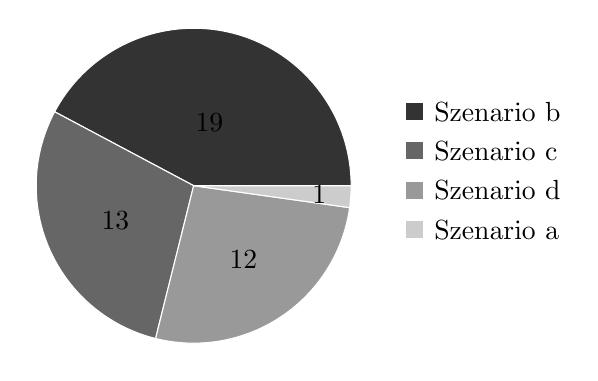
\begin{tikzpicture}
\tikzset{lines/.style={draw=white},}
\pie[color={yellowOfBrevity!80, yellowOfBrevity!60, yellowOfBrevity!40, yellowOfBrevity!20},radius = 2 ,sum=auto, after number=,text=legend,every only number node/.style={text=black},style={lines}]{19/Szenario b,13/Szenario c,12/Szenario d, 1/Szenario a}
\end{tikzpicture}
\caption{Welches war das beste Szenario?}
\label{SzenarioGut}
\end{figure}

Die Mehrheit der Versuchspersonen stimmt mit 19 Stimmen für Szenario \textbf{b} als das beste. \textbf{c} und darauffolgend \textbf{d} liegen im Mittelfeld. Weit abgeschlagen mit nur einer Stimme steht Szenario \textbf{a} auf dem letzten Platz.
       
       
        \begin{figure}[ht]
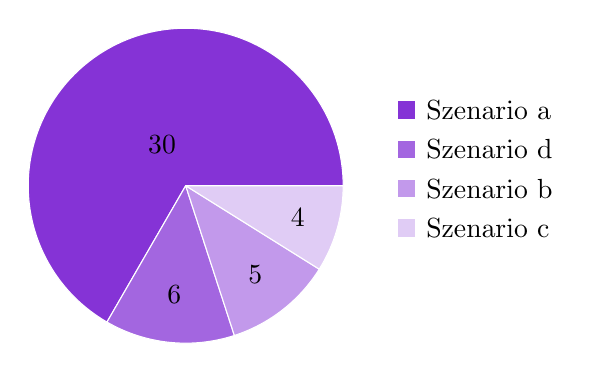
\begin{tikzpicture}
\tikzset{lines/.style={draw=white},}
\pie[color={purpleOfLengthiness!80, purpleOfLengthiness!60, purpleOfLengthiness!40, purpleOfLengthiness!20},radius = 2 ,sum=auto, after number=,text=legend,every only number node/.style={text=black},style={lines}]{30/Szenario a,6/Szenario d,5/Szenario b, 4/Szenario c}
\end{tikzpicture}
\caption{Welches war das schlechteste Szenario?}
\label{SzenarioSchlecht}
\end{figure}
       

Bei der Frage nach dem schlechtesten Szenario sind sich ca. 67\% Prozent der Versuchspersonen einig, dass ihnen \textbf{a} am wenigsten gefallen hat. Deutlich abgeschlagen mit nur 6, 5 und 4 Stimmen die Szenarien \textbf{d}, \textbf{b} und \textbf{c}.
Bei der Sortierung von \textit{gut} nach \textit{schlecht} fällt auf, dass gerade Szenario \textbf{a} wieder eine klare Tendenz hat und es als allgemein schlechter wahrgenommen wurde als alle anderen.

Aus dem Vergleich der beiden Diagramme, die die Befragung der Versuchspersonen nach dem besten (Abb. \ref{SzenarioGut}) und schlechtesten Szenario (Abb. \ref{SzenarioSchlecht}) darstellen, geht Szenario \textbf{a} (Zeitgeber: schnelles Ticken) als eindeutig am schlechtesten bewertetes hervor. Es wurde bei der Frage nach dem besten Szenario am seltesten und bei der Wahl des schlechtesten Szenarios am häufigsten genannt. Dagegen hebt sich das Szenario \textbf{b} (langsames Ticken) positiv hervor; es ist erstplatziert bei der Wahl des besten Szenarios und befindet sich bei der Wahl des schlechtesten auf dem vorletzten Platz. Dies ist gegenteilig wie erwartet, da zuvor vermutet wurde, dass schnelle Zeitgeber auch ein schnelleres Zeitempfinden erzeugen und dieses wiederum auch mit Spaßempfinden verbunden sind.\\
Der These nach, dass das beste Szenario -- das mit dem größten Spaßempfinden -- auch dem als am kürzesten empfunden entspricht, müsste die Reihenfolge der Abb. \ref{SzenarienKurzLang} (Sortierung der Szenarien von kurz nach lang) nun \textbf{b c d a} ergeben. Tatsächlich wurde \textbf{a} jedoch am häufigsten (16 von 48 Einschätzungen) an erster Stelle angegeben, \textbf{b} ist erst an zweiter Stelle zu finden (15 von 47 Einschätzungen).\\
Auch im Vergleich mit den Abb. \ref{SzenarienKurz} und \ref{SzenarienLang} konnte damit die These, dass bei Spaßempfinden die Zeit gefühlt schneller vergeht, in unserem Experiment nicht belegt werden. In den soeben genannten Diagrammen wurde das am schlechtesten empfundene Szenario \textbf{a} als eindeutig kürzestes festgelegt, was bedeutet, dass die kürzeste Zeitspanne in dem Fall am wenigsten Spaß hervorgerufen hat. Das Szenario \textbf{b} wurde bei der Wahl des schnellsten sowie auch der des langsamsten Szenarios an die zweite Stelle gewählt und lässt sich damit nicht sicher einordnen.\\


\section{Diskussion}

Ein Großteil unserer Untersuchungen hat zu keinem eindeutigen Ergebnis geführt. Lediglich die erste unserer drei Hypothesen ("`Visuelle und auditive Zeitgeber verändern das Zeitempfinden der Versuchsperson in der virtuellen Welt'') hat sich zum Teil bestätigt -- insbesondere die auditiven Zeitgeber haben eine Beeinflussung gezeigt. Das Zeitempfinden der Versuchspersonen hat sich nach dem VR-Aufenthalt nur sehr geringfügig verändert und es war keine Beziehung zwischen Spaß- und Zeitempfinden zu erkennen.
 
Ein Grund für die wenigen positiven Ergebnisse kann sein, dass eine größere Anzahl von Versuchspersonen oder zumindest eine gleichmäßigere Verteilung (z.B.\ zwischen dem Männer- und Frauenanteil oder den Altersstufen) notwendig gewesen wäre.

Als Intelligenztest wurde lediglich eine Kurzform verwendet, der zudem stark mit den sprachlichen Fähigkeiten der jeweiligen Versuchsperson zusammenhing (vor allem für Nicht-Muttersprachler eine Schwierigkeit). Es wäre möglich, die Intelligenz vor dem Experiment noch exakter zu überprüfen, auch wenn dies die Gesamtdauer des Experiments erheblich verlängern würde.

Die Einteilung der Müdigkeitsstufen erfolgte nach Selbsteinschätzung, die keine vollkommene Zuverlässigkeit erreichen kann. Hier könnte auf Methoden wie z.B.\ das Zählen von Wimpernschlägen zurückgegriffen werden, um an exaktere Werte zu gelangen.

Auch ungenaue Messungen/Messfehler (z.B.\ bei der Körpertemperatur) können in Einzelfällen nicht ausgeschlossen werden und einen Einfluss auf unser Ergebnis genommen haben.

Eine weiterer Grund für die nicht bestätigten Hypothesen ist, dass die Zeitintervalle der einzelnen Szenarien nicht direkt, während sich die Versuchsperson in der VR-Welt befunden hatte, sondern erst im Nachhinein eingeschätzt werden mussten.
Somit wurde nicht nur die Fähigkeit, Zeit richtig einschätzen zu können, sondern
ebenfalls das Erinnerungsvermögen gefordert, was nicht Ziel unserer Untersuchung sein sollte. Dies sollte bei einer weiteren Durchführung des Experiment unbedingt verändert werden (d.h.\ es sollten unmittelbare Zeiteinschätzungen während des VR-Aufenthalt erfolgen).

Definitiv verändert werden müssen bei einer weiteren Durchführung zudem die gewählten Zeitspannen für Schätzung der Gesamtdauer des VR-Aufenthalts. Eine Versuchsperson hielt sich durchschnittlich 238 Sekunden in der VR-Welt auf -- die erste auswählbare Zeitspanne von 0-7 Minuten war bereits viel zu groß definiert. Dadurch sind die erlangten Ergebnisse nicht aussagekräftig.



\bibliographystyle{plain}
\bibliography{quellen}

\begin{appendix}
\section{Anhang}

\subsection{3D-Objekte}

\subsubsection{American Store}

\textbf{used textures (all licences acquired):}
(last viewed: yyyy-mm-dd)

air\_conditioning:
https://www.textures.com/download/aircos0097/63182?q=air+con
(last viewed: 2017-07-14)

asphalt\_damaged:
https://www.textures.com/download/asphaltdamaged0059/46538?q=asphalt+damaged
(last viewed: 2017-07-14)

back\_door:
https://www.textures.com/download/doorswood0128/64000?q=DoorsWood0128
(last viewed: 2017-07-14)

brown\_concrete:
https://www.textures.com/download/substance0066/128441?q=concrete+brown
(last viewed: 2017-07-14)

concrete\_bare2:
https://www.textures.com/download/concretebare0280/35243?q=ConcreteBare0280
(last viewed: 2017-07-14)

front\_door:
https://www.textures.com/download/doorswood0125/50420?q=door
(last viewed: 2017-07-14)

glas:
https://www.textures.com/download/windowsother0014/44984?q=WindowsOther0014
(last viewed: 2017-07-14)

metal\_plates:
https://www.textures.com/download/metalplatesbare0154/123165?q=MetalPlatesBare0154
(last viewed: 2017-07-14)

plywood\_painted-green:
https://www.textures.com/download/plywoodpainted0024/5719?q=plywood+painted
(last viewed: 2017-07-14)

plywood\_painted-white:
https://www.textures.com/download/plywoodpainted0057/59134?q=plywood+painted+white
(last viewed: 2017-07-14)

rough\_bricks:
https://www.textures.com/download/3dscans0037/126993?q=rough+bricks
(last viewed: 2017-07-14)

rubber:
https://www.textures.com/download/rubber0044/58887?q=Rubber0044
(last viewed: 2017-07-14)

shutter:
https://www.textures.com/download/windowsshutters0096/31421?q=WindowsShutters0096
(last view: 2017-07-14)

soilsand:
https://www.textures.com/download/soilsand0210/61549?q=soilsand0210
(last viewed: 2017-07-14)
---
\textbf{used normalmap:}

all normalmaps were created out of the respective textures using 'http://cpetry.github.io/NormalMap-Online/'
(last viewed: 2017-07-14)

\subsubsection{Straßenverkehr}

strassenoberfläche:
http://www.bildburg.de/texturen/boden/strassen/
(last viewed: 2017-07-20)


%%%%%%%%%%%%%%%%% Alinas Texturen %%%%%%%%%%%%%%%%%%%%%%%%%%%%%%%%% 
https://pixabay.com/de/textur-stamm-holz-nahaufnahme-1411201/



https://pixabay.com/de/textur-baum-rinde-hintergrund-2119288/



https://pixabay.com/de/mauer-steine-wand-hauswand-450106/



https://pixabay.com/de/wand-putz-hintergrund-fassade-2146911/



https://pixabay.com/de/t\%C3\%BCr-alt-eingang-die-alte-t\%C3\%BCr-2166761/



https://pixabay.com/de/die-t\%C3\%BCr-holz-burg-blumen-t\%C3\%BCrgriff-1908710/



https://pixabay.com/de/die-t\%C3\%BCr-holz-burg-blumen-t\%C3\%BCrgriff-1909077/



https://pixabay.com/de/dach-ziegel-bunt-rot-dachplatten-1197886/



https://pixabay.com/de/dachziegel-dachpfannen-dach-707888/



https://pixabay.com/de/dachziegel-dachpfannen-dach-1301459/



https://pixabay.com/de/dach-bretter-holzwand-holz-2071600/



https://pixabay.com/de/hauswand-ziegelsteine-backsteine-298039/



https://pixabay.com/de/steinwand-stein-mauer-wand-2370933/



https://pixabay.com/de/blatt-gr\%C3\%BCn-gr\%C3\%BCnes-blatt-910532/



https://pixabay.com/de/herbst-herbstbl\%C3\%A4tter-laub-1655915/



https://pixabay.com/de/erdbeeren-erdbeere-lecker-obst-1326148/



https://pixabay.com/de/gem\%C3\%BCse-gurke-tomaten-kirschtomate-1940461/

\end{appendix}

\vfill %Zum Seitenende Verschieben


\end{document}
